% =====================================================================
%  Construção de Banco de Dados --- UFRJ
%  Tarefa: Dispositivos de Armazenamento Físico para SBD
%  Versão condensada (revisão de 11/09/2026)
% =====================================================================
\documentclass[11pt,a4paper]{article}

\usepackage[T1]{fontenc}
\usepackage[utf8]{inputenc}
\usepackage[portuges]{babel}
\usepackage{lmodern}
\usepackage{amsmath,amssymb}
\usepackage[a4paper,left=2.6cm,right=2.4cm,top=2.6cm,bottom=2.4cm]{geometry}
\usepackage{booktabs,longtable,array,tabularx,multirow,makecell}
\usepackage{graphicx,xcolor,microtype,enumitem,ragged2e,float}
\usepackage{pdflscape}
\usepackage{caption}
\usepackage{fancyhdr}
\usepackage{titlesec}
\usepackage{xurl}
\usepackage[hidelinks]{hyperref}
\setlength{\emergencystretch}{2em}
\setcounter{tocdepth}{2}

\definecolor{azul}{HTML}{2A78D6}
\definecolor{laranja}{HTML}{EB6834}
\definecolor{tinta}{HTML}{0B0B0B}
\definecolor{tinta2}{HTML}{52514E}
\definecolor{linha}{HTML}{E3E2DE}
\definecolor{fundo}{HTML}{F6F6F4}

\hypersetup{colorlinks=true,linkcolor=azul,urlcolor=azul,citecolor=azul}

\captionsetup{font=small,labelfont={bf,color=tinta},textfont={color=tinta2},
              justification=justified,singlelinecheck=false,skip=6pt}

\titleformat{\section}{\Large\bfseries\color{tinta}}{\thesection}{0.6em}{}
\titleformat{\subsection}{\large\bfseries\color{tinta}}{\thesubsection}{0.6em}{}
\titleformat{\subsubsection}{\normalsize\bfseries\color{tinta2}}{\thesubsubsection}{0.6em}{}
\titlespacing*{\section}{0pt}{16pt}{6pt}
\titlespacing*{\subsection}{0pt}{12pt}{5pt}
\titlespacing*{\subsubsection}{0pt}{10pt}{3pt}

\pagestyle{fancy}\fancyhf{}
\fancyhead[L]{\footnotesize\color{tinta2}Armazenamento Físico para SBD --- CBD/UFRJ}
\fancyhead[R]{\footnotesize\color{tinta2}\thepage}
\renewcommand{\headrulewidth}{0.4pt}
\renewcommand{\headrule}{\color{linha}\hrule height 0.4pt}

\setlist{itemsep=1pt,parsep=0pt,topsep=3pt}
\setlength{\parskip}{4pt}
\setlength{\parindent}{0pt}
\renewcommand{\arraystretch}{1.15}

% caixas de destaque
\newcommand{\destaque}[2]{%
  \begin{center}\begin{minipage}{0.97\textwidth}
  \colorbox{fundo}{\begin{minipage}{\dimexpr\linewidth-2\fboxsep}
  \vspace{3pt}\textbf{\color{azul}#1}\\[2pt]\small #2\vspace{3pt}
  \end{minipage}}\end{minipage}\end{center}}

\newcommand{\correcao}[2]{%
  \begin{center}\begin{minipage}{0.97\textwidth}
  \colorbox{fundo}{\begin{minipage}{\dimexpr\linewidth-2\fboxsep}
  \vspace{3pt}\textbf{\color{laranja}#1}\\[2pt]\small #2\vspace{3pt}
  \end{minipage}}\end{minipage}\end{center}}

\newcommand{\us}{\,\textmu s}

\begin{document}

% =====================================================================
% FOLHA DE ROSTO
% =====================================================================
\thispagestyle{empty}
\begin{center}
\vspace*{0.6cm}
{\large\scshape Universidade Federal do Rio de Janeiro}\\[2pt]
{\normalsize Instituto de Matemática --- Departamento de Ciência da Computação}\\[2pt]
{\normalsize Disciplina: \textbf{Construção de Banco de Dados}}\\[2pt]
{\normalsize Professor: Milton Ramirez}\\[1.6cm]

{\color{linha}\rule{\textwidth}{1.2pt}}\\[0.7cm]
{\LARGE\bfseries Dispositivos de Armazenamento Físico\\[6pt] para Sistemas de Banco de Dados}\\[0.5cm]
{\large Interfaces de Conexão e Parâmetros para o\\ Gerente de Armazenamento do SBD}\\[0.5cm]
{\normalsize\itshape Atualização da Tabela 16.1 (Elmasri \& Navathe, 7\textsuperscript{a} ed.)\\ dados consultados em 05 de setembro de 2026}\\[0.6cm]
{\color{linha}\rule{\textwidth}{1.2pt}}\\[1.4cm]

{\large\bfseries Integrantes do Grupo}\\[0.5cm]
\begin{minipage}{0.85\textwidth}\centering
\begin{tabular}{@{}p{9.2cm}p{3.4cm}@{}}
\toprule
\textbf{Nome completo} & \textbf{DRE} \\
\midrule
Bernardo Brandão Pozzato Carvalho Costa & 123289593 \\
Enzo de Carvalho Sampaio & 123386206 \\
Gabriel Schmitz Corrêa Rizawinsk & 123225573 \\
Guilherme En Shih Hu & 123224674 \\
Raphael Henrique da Silva Pereira & 123420783 \\
Vivian Maria da Silva e Souza & 123205793 \\
\bottomrule
\end{tabular}
\end{minipage}

\vfill
{\normalsize Rio de Janeiro --- Setembro de 2026}
\end{center}
\newpage

% =====================================================================
\thispagestyle{empty}
\section*{Resumo}
\addcontentsline{toc}{section}{Resumo}

Este trabalho estuda os dispositivos de armazenamento físico para Sistemas de Banco de Dados
(SBD), suas interfaces de conexão e os parâmetros que interessam ao \emph{Gerente de
Armazenamento}, a partir de Elmasri \& Navathe (Cap.~16), Silberschatz, Korth \& Sudarshan
(Cap.~12) e Garcia-Molina, Ullman \& Widom (Cap.~13). Três produtos atendem ao enunciado:
\textbf{(i)}~uma revisão dos fundamentos (hierarquia de memória, disco magnético, \emph{flash},
memória de classe de armazenamento, fita e mídia óptica); \textbf{(ii)}~a \textbf{atualização
da Tabela~16.1} com produtos comerciais de 2026, largura de banda segregada em leitura e
escrita, faixas de preço e a nova coluna de \textbf{preço por kilobyte}; e \textbf{(iii)}~uma
\textbf{tabela comparativa das interfaces} USB, SCSI, SATA, eSATA, SATA Express, SAS,
PCIe/NVMe (M.2, U.2, U.3, EDSFF), NVMe-oF, iSCSI, FireWire, HBA, Fibre Channel (com FCIP e
FCoE) e InfiniBand.

Três achados orientam o texto. Primeiro, a memória persistente endereçável por byte
\textbf{saiu do mercado} com a descontinuação do Intel Optane, e o vão de quase três ordens
de grandeza entre DRAM ($\approx$70\,ns) e SSD NVMe ($\approx$50\us) só é coberto em parte por
módulos CXL, medidos em 214--271\,ns. Segundo, SSD e HDD \textbf{divergiram em custo por
terabyte}: a razão foi de 7$\times$ no 3\textsuperscript{o} trimestre de 2025 a 23,2$\times$
no 1\textsuperscript{o} de 2026, e estava em 18,6$\times$ em 05/09/2026. Terceiro, o
desempenho de um SBD transacional depende de \textbf{latência e profundidade de fila} mais
do que de largura de banda, o que explica a estagnação do SATA em 6\,Gb/s e a vitória do
NVMe. A Seção~9 traz o \textbf{Post-Mortem} exigido: prompts-chave, autoria e registro dos
erros da IA com as correções, incluindo a correção da afirmação do enunciado de que ``SATA
também é conhecida como NL-SAS''.

\vspace{0.4cm}
\textbf{Palavras-chave:} hierarquia de memória; SSD NVMe; HAMR; LTO-10; CXL; Fibre Channel;
InfiniBand; gerente de armazenamento; latência de \emph{commit}.

\newpage
\thispagestyle{empty}
{\small\setlength{\parskip}{0pt}\tableofcontents}
\newpage
\setcounter{page}{1}

% =====================================================================
\section{Introdução}

Organização de arquivos, índices B\textsuperscript{+}-tree, otimização de consultas e
recuperação existem porque o meio persistente é ordens de grandeza mais lento que a memória
principal: o otimizador conta \emph{blocos lidos}, o \emph{buffer pool} evita releituras e o
\emph{log} de escrita antecipada (WAL) torna sequencial a escrita que garante durabilidade. A
razão entre essas velocidades, que justifica toda essa arquitetura, \textbf{mudou por várias
ordens de grandeza} desde que os livros-texto foram escritos. A Tabela~16.1 de Elmasri \&
Navathe traz preços de 2014 e o Capítulo~12 de Silberschatz, números de 2018. Em 2026 o disco
magnético deixou de ser o meio principal dos bancos de produção, a memória persistente foi
descontinuada e o barramento deixou de ser gargalo. Este trabalho mede essa distância.

\subsection{Objetivos e organização}

Os três objetivos do enunciado ocupam as Seções~2 (fundamentos), 3 (Tabela~16.1 atualizada)
e 4 (interfaces de conexão). Por iniciativa do grupo, a Seção~5 traduz os números em
\textbf{parâmetros acionáveis para o Gerente de Armazenamento} (tamanho de bloco,
\emph{buffer pool}, latência de \emph{commit}, modelo de custo e \emph{tiering}). As
Seções~6 e~7 trazem a conclusão e os pontos para o debate, e a Seção~9, o Post-Mortem do uso
de IA generativa.

\subsection{Metodologia e critérios de seleção}

A pesquisa combinou três tipos de fonte. \textbf{(a)~Livros-texto}: Elmasri \& Navathe
fornecem a Tabela~16.1 e as arquiteturas modernas (SAN, NAS, iSCSI, \emph{tiering});
Silberschatz \emph{et al.} detalham a física do \emph{flash}, a FTL e as métricas de disco;
Garcia-Molina, Ullman \& Widom formalizam o \emph{I/O model of computation}, usado na
Seção~5.4. \textbf{(b)~Especificações normativas} de USB-IF, SATA-IO, INCITS/T10 e T11,
NVM Express, PCI-SIG, IEEE, IETF, IBTA, CXL Consortium, SNIA e LTO Program.
\textbf{(c)~Documentação de fabricante} e preços de referência consultados em 05/09/2026.
Para escolher os dispositivos da Tabela~16.1 atualizada, adotamos três critérios, nesta ordem:

\begin{enumerate}[label=\textbf{C\arabic*.}]
\item \textbf{Disponibilidade das quatro informações do enunciado} (capacidade, tempo de
      acesso, largura de banda e preço).
\item \textbf{Representatividade de mercado}: produto em produção corrente, com preço
      público verificável.
\item \textbf{Rastreabilidade}: cada célula tem origem declarada (\emph{datasheet}, medição
      de terceiro, derivação aritmética ou estimativa).
\end{enumerate}

\destaque{Convenção de unidades}{%
Distinguimos \textbf{bit} (b) de \textbf{byte} (B): 1\,GB/s $=$ 8\,Gb/s. Capacidades de
armazenamento seguem a convenção decimal da indústria (1\,TB $=$ 10\textsuperscript{12}\,B);
memórias (SRAM, DRAM) seguem a binária JEDEC. Para a coluna de preço por KB, toda capacidade
é convertida em bytes e dividida por 1\,KB $=$ 1.000\,B (Nota~N1 da Tabela~\ref{tab:161}).}

% =====================================================================
\section{Fundamentos dos Sistemas de Armazenamento Físico para SBD}

\subsection{A hierarquia de memória}

Silberschatz \emph{et al.} (Figura~12.1) ordenam os meios por velocidade e custo:
\emph{cache}, memória principal, \emph{flash}, disco magnético, disco óptico e fita. Elmasri
\& Navathe agrupam essa ordem em três estratos:

\begin{itemize}
\item \textbf{Primário}: \emph{cache} SRAM e DRAM, operáveis diretamente pela CPU e
      \textbf{voláteis}.
\item \textbf{Secundário} (\emph{online}): SSD e disco magnético, \textbf{não voláteis} e de
      acesso direto a qualquer bloco.
\item \textbf{Terciário} (\emph{offline}): mídia óptica e fita, em geral removíveis; a fita
      tem \textbf{acesso sequencial}.
\end{itemize}

Cada nível só existe porque ocupa um ponto não dominado da fronteira
custo\,$\times$\,velocidade: se um meio fosse ao mesmo tempo mais rápido e mais barato que
outro, o mais lento desapareceria. A Figura~\ref{fig:hier} mostra que essa fronteira continua
valendo em 2026, com um \textbf{vão} entre os níveis primário e secundário (Seção~2.5).

\begin{figure}[H]\centering
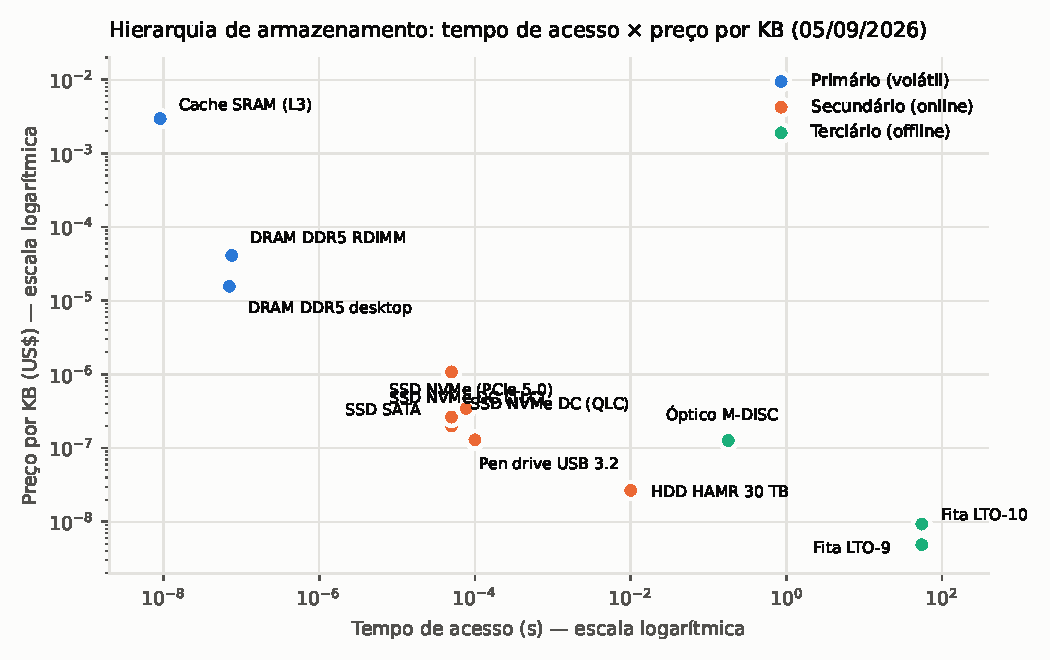
\includegraphics[width=0.80\textwidth]{fig/fig1_hierarquia.pdf}
\caption{Tecnologias da Tabela~\ref{tab:161} por tempo de acesso e preço por kilobyte
(escalas logarítmicas). Pagar mais compra latência menor. Entre a DRAM
($\sim$10\textsuperscript{-7}\,s) e o SSD NVMe ($\sim$5\,$\times$\,10\textsuperscript{-5}\,s)
há um vão de quase três ordens de grandeza, o degrau que o Intel Optane ocupava.}
\label{fig:hier}
\end{figure}

\subsection{Volatilidade e durabilidade}

A distinção volátil/não volátil sustenta a propriedade \textbf{D} do ACID: um
\texttt{COMMIT} só pode ser confirmado depois que os dados de recuperação chegam a um meio
que sobrevive a uma queda de energia. O WAL barateia essa travessia trocando escritas
espalhadas de páginas por um registro sequencial pequeno. Por isso, para um SGBD
transacional, o parâmetro decisivo de um dispositivo é a \textbf{latência de uma escrita
sincronizada pequena} (o custo de um \texttt{fsync}), e não sua largura de banda
(Seção~5.3).

\subsection{Disco magnético}

O disco rígido é o componente eletromecânico mais comum no caminho de dados \emph{online}, e
sua mecânica define os parâmetros clássicos dos modelos de custo:

\begin{itemize}
\item \textbf{Tempo de busca}: 2 a 20\,ms conforme a distância, com médias de 4 a 10\,ms
      (Silberschatz).
\item \textbf{Latência rotacional}: meia volta em média; a 7.200\,rpm, uma volta leva
      8,33\,ms e a média é $\approx$4,17\,ms (a Seagate publica 4,16\,ms para o Exos~M).
\item \textbf{Taxa de transferência}: 50 a 200\,MB/s em Silberschatz (2018); discos HAMR de
      2026 chegam a 275--285\,MB/s nas trilhas externas.
\item \textbf{IOPS}: 50 a 200 com blocos de 4\,KB, praticamente o mesmo valor de duas
      décadas atrás, porque é limitado pela mecânica e não pela densidade.
\end{itemize}

\destaque{O que os livros-texto não enfatizam}{%
A capacidade do HDD cresceu 4 a 4,5$\times$ desde 2014 (8\,TB $\rightarrow$ 32--36\,TB), a
taxa sequencial 1,4$\times$ (200 $\rightarrow$ 275\,MB/s) e o IOPS ficou constante. Ler o disco
inteiro passou de $\approx$11\,h (8\,TB a 200\,MB/s) para $\approx$32\,h (32\,TB a
275\,MB/s). Janelas de \emph{backup}, reconstrução de RAID e varreduras completas
\textbf{pioraram}, e por isso o RAID~5 deixou de ser recomendado para discos de alta
capacidade (Seção~2.7).}

\subsection{Memória flash e SSD}

A NAND organiza-se em \textbf{páginas} de $\approx$4\,KB agrupadas em \textbf{blocos de
apagamento} de 256\,KB a 1\,MB. Ler uma página leva dezenas de microssegundos e escrever
numa página apagada, $\approx$100\us; \textbf{sobrescrever é impossível}: é preciso apagar o
bloco inteiro (2 a 5\,ms), consumindo um dos 10\textsuperscript{5}--10\textsuperscript{6}
ciclos de vida. A \emph{Flash Translation Layer} (FTL) contorna isso redirecionando cada
atualização para uma página já apagada; o \emph{garbage collection} recupera blocos com
páginas inválidas e o \emph{wear leveling} distribui o desgaste. Acima da FTL, o SSD expõe a
mesma interface de blocos de um disco (Silberschatz, §12.4).

\destaque{Três consequências para o projeto de SBD}{%
\textbf{(1)~Amplificação de escrita}: o \emph{garbage collection} move dados, e estruturas com
atualização no lugar (B\textsuperscript{+}-tree) sofrem mais que estruturas
\emph{append-only} (LSM-tree), adotadas por RocksDB, Cassandra e ScyllaDB.
\textbf{(2)~Latência de cauda}: a mediana é excelente, mas o percentil 99,9 pode ser dez
vezes pior, e SLAs quebram na cauda. \textbf{(3)~Paralelismo interno}: um SSD SATA entrega
$\approx$13\,mil IOPS a QD$=$1 e $\approx$98\,mil a QD$=$32; emitir uma requisição por vez
desperdiça o dispositivo.}

O desgaste é especificado em \textbf{DWPD} (escritas do disco inteiro por dia) ou
\textbf{TBW}. Um SSD de 61,44\,TB com 0,6~DWPD em cinco anos admite
$0{,}6 \times 61{,}44\,\text{TB} \times 365 \times 5 \approx 67$\,PB escritos. Um SGBD com
\emph{log} intensivo pode esgotar a resistência antes da capacidade.

\subsection{Memória de classe de armazenamento e CXL}

A Nota~12.1 de Silberschatz apresenta a \emph{storage class memory} (SCM): memória não volátil
endereçável por byte, cujo exemplo é o 3D~XPoint, vendido como \textbf{Intel Optane} em SSD
(2017) e em módulos DIMM de memória persistente (2018).

\correcao{Atualização: a categoria foi extinta comercialmente}{%
A Intel anunciou a saída do negócio Optane em \textbf{julho de 2022}; a geração 300
(\emph{Crow Pass}) foi cancelada e os últimos embarques da série 200 estavam previstos para o
\textbf{fim de 2025}. Em setembro de 2026 \textbf{não há memória persistente endereçável por
byte de uso geral em produção}, e o degrau da Nota~12.1 desapareceu.}

O substituto parcial é o \textbf{CXL} (\emph{Compute Express Link}), protocolo coerente sobre
a camada física do PCIe. Um módulo CXL Tipo~3, como o Samsung CMM-D MD220 (E3.S, PCIe~Gen5),
acrescenta DRAM ao sistema, mas é volátil e mais lento que a DRAM local:
medições independentes em expansores CXL~2.0 dão \textbf{214--271\,ns}, contra 111--117\,ns
da DDR5 local, isto é, 2 a 2,5$\times$ (origem e ressalvas na Nota~N5). O CXL~3.2 (dez./2024)
introduziu a \emph{Hot-Page Monitoring Unit}, que permite ao SO ou ao SGBD promover páginas
quentes para a DRAM local e rebaixar as frias. Para um banco de dados, isso significa
\emph{buffer pool} maior e, portanto, menos I/O.

\subsection{Fita e mídia óptica: o estrato terciário}

\textbf{Fita.} Os livros subestimam a tecnologia (Silberschatz cita 1--12\,TB; a Tabela~16.1,
2,5--8,5\,TB). O padrão corrente é o \textbf{LTO-10}: especificado com 30\,TB nativos em
2025, ganhou um cartucho de \textbf{40\,TB nativos} (especificação de nov./2025, embarques
desde jan./2026) compatível com os \emph{drives} existentes. A taxa nativa continua em
\textbf{400\,MB/s}, igual à do LTO-9 e acima da de um HDD, e a mídia custa $\approx$US\$\,5--10
por TB. O \emph{roadmap} foi revisado para baixo em novembro de 2025 e termina em
\textbf{365\,TB nativos} no LTO-14; os 913\,TB que circulam são capacidade comprimida a
2,5:1 (erro E13). A fita sobrevive porque \emph{drive} e mídia têm preços separados (cada TB
adicional é barato), porque não consome energia na estante, porque a desconexão física
(\emph{air gap}) protege contra \emph{ransomware} e porque a retenção declarada é de 30 anos.
Para o SBD, é a última linha do plano de recuperação de desastres.

\textbf{Óptico.} A categoria está em colapso comercial: a Pioneer encerrou a fabricação de
\emph{drives} ópticos para PC em maio de 2025 e a Sony encerrou o \emph{Optical Disc Archive}
em 31/03/2025. Resta o nicho WORM de longuíssimo prazo, representado pelo M-DISC BD-XL de
100\,GB, de interesse para retenção legal.

\subsection{RAID e otimizações de acesso a bloco}

Com MTTF de 100.000\,h por disco, 100 discos têm MTTF agregado de 1.000\,h ($\approx$41 dias),
o que torna a redundância obrigatória (Silberschatz, §12.5). O \textbf{RAID~1} espelha, com
100\% de \emph{overhead} e boa escrita; o \textbf{RAID~5} usa um disco de paridade, mas cada
escrita lógica custa \textbf{quatro I/Os} (ler dado e paridade antigos, escrever ambos).
Por isso a recomendação clássica põe o \emph{log} em RAID~1 e os dados em RAID~5 ou~10. Com
discos de 30\,TB, reconstruções de mais de 30\,h tornam o RAID~5 contraindicado; RAID~6 ou
\emph{erasure coding} são o padrão.

Das otimizações de §12.6, o \emph{buffering} ganhou importância (a memória cresceu mais que o
custo de acessá-la); o \emph{read-ahead} segue útil em varreduras; o escalonamento de braço
só vale para HDD; \emph{extents} continuam reduzindo metadados; e os \emph{buffers} de escrita
não voláteis (NVRAM) seguem essenciais para confirmar escritas sem violar a durabilidade.

\correcao{Armadilha de durabilidade}{%
Uma controladora RAID com \emph{cache} de escrita sem proteção por bateria ou \emph{flash}
pode confirmar um \texttt{fsync} antes de persistir o dado, e muitas pontes USB--SATA não
implementam corretamente o comando FUA (\emph{Force Unit Access}). É o argumento técnico, e
não só de desempenho, para \textbf{não} colocar dados de produção atrás de USB.}

% =====================================================================
\section{A Tabela 16.1 Atualizada para 2026}

\subsection{A tabela original e o que se pede}

A Tabela~16.1 de Elmasri \& Navathe (final da Seção~16.1.1), com preços de \textbf{2014}:

\begin{center}\footnotesize
\setlength{\tabcolsep}{3pt}
\begin{tabular}{@{}lllll@{}}
\toprule
\textbf{Type} & \textbf{Capacity} & \textbf{Access Time} & \textbf{Max Bandwidth} & \textbf{Commodity Prices (2014)} \\
\midrule
Main Memory --- RAM        & 4\,GB--1\,TB      & 30\,ns     & 35\,GB/s                & US\$100--20\,K \\
Flash Memory --- SSD       & 64\,GB--1\,TB     & 50\us & 750\,MB/s            & US\$50--600 \\
Flash Memory --- USB stick & 4\,GB--512\,GB    & 100\us & 50\,MB/s            & US\$2--200 \\
Magnetic Disk              & 400\,GB--8\,TB    & 10\,ms     & 200\,MB/s               & US\$70--500 \\
Optical Storage            & 50\,GB--100\,GB   & 180\,ms    & 72\,MB/s                & US\$100 \\
Magnetic Tape              & 2,5\,TB--8,5\,TB  & 10--80\,s  & 40--250\,MB/s           & US\$2,5\,K--30\,K \\
Tape jukebox               & 25\,TB--2,1\,EB   & 10--80\,s  & 250\,MB/s--1,2\,PB/s    & US\$3\,K--1\,M+ \\
\bottomrule
\end{tabular}
\end{center}

O enunciado pede: trocar cada tipo por \textbf{exemplos comerciais atuais}, atualizar
capacidade e \textbf{faixa de preço}, \textbf{segregar a banda em leitura e escrita} quando
houver o dado, acrescentar a coluna de \textbf{preço por kilobyte} e manter o tempo de acesso
do livro quando não houver valor. Por iniciativa do grupo, acrescentamos a coluna de exemplo
comercial e \textbf{quatro linhas} (CXL, SSD NVMe \emph{datacenter} QLC e TLC, LTO-10),
justificadas na Seção~3.2.

\subsection{Linhas acrescentadas e removidas}

A linha de \textbf{CXL} entrou porque é o único candidato ao vão deixado pelo Optane. A linha
``SSD'' do livro foi \textbf{desdobrada em três} (consumidor PCIe~5.0, \emph{datacenter} QLC
e TLC) porque esconde duas ordens de grandeza em capacidade (1 a 122,88\,TB), mais de
5$\times$ em preço por byte e uma decisão real de projeto entre capacidade e desempenho. A
fita foi desdobrada em \textbf{LTO-9 e LTO-10} porque a transição está em curso. Ficaram de
fora o \textbf{Intel Optane} e o \textbf{Sony Optical Disc Archive}, ambos descontinuados
(critério C2); a ausência do Optane é tratada como achado (Seção~2.5).

\subsection{Tabela 16.1 atualizada --- consulta em 05/09/2026}

A Tabela~\ref{tab:161}, na página seguinte, deve ser lida com as notas N1--N8, que registram a origem de cada
número. Onde não havia dado confiável, a célula traz ``n/d''. A coluna de preço por KB varre
seis ordens de grandeza, de $3{,}0\times10^{-3}$ (SRAM) a $4{,}9\times10^{-9}$ (LTO-9), uma
razão de $\approx$607 mil vezes.

\newgeometry{landscape,left=1.6cm,right=1.6cm,top=1.3cm,bottom=1.3cm}
\begin{landscape}
\thispagestyle{empty}
{\footnotesize
\setlength{\tabcolsep}{4pt}
\renewcommand{\arraystretch}{1.0}
\begin{longtable}{@{}>{\RaggedRight\arraybackslash}p{3.4cm}>{\RaggedRight\arraybackslash}p{4.3cm}>{\RaggedRight\arraybackslash}p{2.4cm}>{\RaggedRight\arraybackslash}p{2.3cm}>{\RaggedRight\arraybackslash}p{2.2cm}>{\RaggedRight\arraybackslash}p{2.2cm}>{\RaggedRight\arraybackslash}p{3.1cm}>{\RaggedRight\arraybackslash}p{1.9cm}@{}}
\caption{\textbf{Tabela 16.1 atualizada.} Capacidade, tempo de acesso, banda segregada em
leitura e escrita, preço de referência e preço por kilobyte decimal. Consulta: 05/09/2026.
Linhas marcadas com [nova] não existem no original. Origem de cada valor nas notas N1--N8.}\label{tab:161}\\
\toprule
\textbf{Tipo} & \textbf{Exemplo comercial (2026)} & \textbf{Capacidade} &
\textbf{Tempo de acesso} & \textbf{Banda máx.\ leitura} & \textbf{Banda máx.\ escrita} &
\textbf{Preço (US\$)} & \textbf{Preço/KB (US\$)} \\
\midrule
\endfirsthead
\toprule
\textbf{Tipo} & \textbf{Exemplo comercial (2026)} & \textbf{Capacidade} &
\textbf{Tempo de acesso} & \textbf{Banda máx.\ leitura} & \textbf{Banda máx.\ escrita} &
\textbf{Preço (US\$)} & \textbf{Preço/KB (US\$)} \\
\midrule
\endhead
\bottomrule
\endfoot

\textbf{Cache SRAM (L3)} &
AMD Ryzen 9 9950X3D2 (3D V-Cache) / EPYC 9755 &
96\,MB--512\,MB &
$\approx$9,0\,ns$^{\ddagger}$ \newline (L1 0,71; L2 2,50) &
$\approx$1,4\,TB/s por CCD &
$\approx$1,4\,TB/s &
700--14.800 \newline (preço da CPU; N2) &
$3{,}0\times10^{-3}$ \\

\textbf{DRAM (desktop)} &
Corsair Vengeance DDR5-6000 CL30, kit 2$\times$16\,GB &
16--96\,GB (kit) &
70\,ns efetivo \newline (CAS 10,0\,ns) &
96\,GB/s (2 canais) &
96\,GB/s &
270--1.100 &
$1{,}6\times10^{-5}$ \\

\textbf{DRAM (servidor)} &
RDIMM DDR5-6400 64\,GB (Kingston / A-Tech) &
32--256\,GB por módulo &
$\approx$75\,ns &
51,2\,GB/s por módulo \newline (614\,GB/s por soquete, 12 canais) &
51,2\,GB/s &
1.000--4.000 por módulo &
$4{,}1\times10^{-5}$ \\

\textbf{Memória CXL 2.0 (Tipo 3)} [nova] &
Samsung CMM-D MD220 (E3.S, PCIe Gen5) &
128--256\,GB &
214--271\,ns$^{\dagger}$ \newline (2--2,5$\times$ a DRAM local) &
$\approx$36\,GB/s$^{\dagger}$ &
$\approx$36\,GB/s$^{\dagger}$ &
não público \newline (canal OEM) &
n/d \\

\textbf{SSD NVMe PCIe 5.0 (consumidor)} &
Samsung 9100 PRO 1\,TB (M.2 2280) &
1--8\,TB (dados: 1\,TB) &
50\us{} (livro) &
14,7\,GB/s \newline (1,85\,M IOPS) &
13,3\,GB/s \newline (2,60\,M IOPS) &
199,99 (1\,TB, MSRP) &
$2{,}0\times10^{-7}$ \\

\textbf{SSD NVMe \emph{datacenter} QLC} [nova] &
Solidigm D5-P5336 (U.2 / E3.S / E1.L) &
7,68--122,88\,TB &
50\us{} (livro) &
7,0\,GB/s \newline (900\,K IOPS) &
3,0\,GB/s &
16.246--33.249 \newline (61,44\,TB) &
$2{,}6\times10^{-7}$ \\

\textbf{SSD NVMe \emph{datacenter} TLC} [nova] &
Micron 9550 PRO (E1.S / U.2, PCIe 5.0) &
7,68--30,72\,TB &
50\us{} (livro) &
14,0\,GB/s \newline (3,3\,M IOPS) &
10,0\,GB/s &
33.217 (30,72\,TB, lista) &
$1{,}1\times10^{-6}$ \\

\textbf{SSD SATA} &
Samsung 870 EVO (2,5 polegadas) &
250\,GB--4\,TB &
77\us{} leitura \newline 28\us{} escrita &
560\,MB/s &
530\,MB/s &
345 (1\,TB) &
$3{,}4\times10^{-7}$ \\

\textbf{Pen drive USB} &
Kingston DataTraveler Max (USB 3.2 Gen 2) &
256\,GB--1\,TB &
100\us{} (livro) &
1.000\,MB/s &
900\,MB/s &
130 (1\,TB) &
$1{,}3\times10^{-7}$ \\

\textbf{Disco magnético HAMR} &
Seagate Exos M 30\,TB (ST30000NM004K) &
24--36\,TB \newline (44\,TB anunciado) &
10\,ms (livro) &
275\,MB/s sustentado &
275\,MB/s &
800 (30\,TB) --- 1.280 (32\,TB) &
$2{,}7\times10^{-8}$ \\

\textbf{Óptico WORM} &
Verbatim M-DISC BD-XL 100\,GB $+$ Pioneer BDR-X13U &
100\,GB por disco &
180\,ms (livro) &
não publicada \newline ($\approx$36\,MB/s no leitor, 8$\times$) &
$\approx$18\,MB/s (4$\times$) &
12,70 por disco \newline $+$ 230 (leitor) &
$1{,}3\times10^{-7}$ \\

\textbf{Fita LTO-9} &
Cartucho LTO-9 Ultrium (HPE / Fujifilm / IBM) &
18\,TB nativo \newline (45\,TB comp.) &
25--121\,s \newline (carga $+$ \emph{locate}) &
400\,MB/s nativo \newline (1.000 comp.) &
400\,MB/s nativo &
88 por cartucho \newline $+$ 4\,K--6\,K (\emph{drive}) &
$4{,}9\times10^{-9}$ \\

\textbf{Fita LTO-10} [nova] &
Cartucho LTO-10 Ultrium (Fujifilm, jan./2026) &
30\,TB $\rightarrow$ 40\,TB nativo &
25--121\,s &
400\,MB/s nativo \newline (1.200 comp., FC) &
400\,MB/s nativo &
260--300 por cartucho \newline $+$ $\approx$24\,K (\emph{drive}) &
$9{,}3\times10^{-9}$ \newline (30\,TB) \\

\textbf{\emph{Tape library}} &
IBM TS4500 (23.170 cartuchos) / Quantum Scalar i6000 &
até 926,8\,PB nativo \newline (2,317\,EB a 2,5:1) &
25--121\,s &
$\approx$51,2\,GB/s agregado (128 \emph{drives}) &
$\approx$51,2\,GB/s &
sob cotação \newline (não publicado) &
n/d \\
\end{longtable}
}
\end{landscape}
\restoregeometry

\subsubsection*{Notas da Tabela~\ref{tab:161}}

{\small
\begin{enumerate}[label=\textbf{N\arabic*.},leftmargin=*]
\item \textbf{Preço por KB.} Capacidade em bytes dividida por 1\,KB $=$ 1.000\,B, usando o
      preço e a capacidade pontuais de cada linha (não os extremos das faixas). Ex.: SRAM,
      64\,MiB $=$ 67.108,864\,KB e US\$\,199 $\Rightarrow$ $2{,}97\times10^{-3}$; LTO-10
      calculado com o cartucho de 30\,TB. No 9100 PRO, preço (MSRP de lançamento, US\$\,199,99)
      e desempenho são ambos do modelo de 1\,TB; o de 4\,TB chega a 14.800\,MB/s e
      2.200\,KIOPS de leitura (erro E20). MSRP é referência histórica, não cotação atual.
\item \textbf{SRAM é \emph{proxy}.} \emph{Cache} não é vendido isoladamente; o valor é o
      \emph{delta} de preço entre CPUs com e sem V-Cache. Embute margem e segmentação e vale
      só como ordem de grandeza ($\approx$72$\times$ o preço por byte da DRAM de servidor).
\item \textbf{Tempo de acesso do \emph{cache} ($\ddagger$) é derivação.} A AMD publica
      L1D $=$ 4 ciclos (Zen~5) e, para o L3, apenas ``3,5 ciclos a menos'' que os 50 do Zen~4
      ($\Rightarrow$ 46,5); o L2 de 14 ciclos é do Zen~4. Com o \emph{clock} de 5,6\,GHz:
      $4/5{,}6=0{,}71$\,ns, $14/5{,}6=2{,}50$\,ns e $46{,}5/5{,}6=8{,}30$\,ns, mais $\approx$0,71\,ns
      do V-Cache empilhado $\Rightarrow$ $\approx$9,0\,ns. Nenhum desses valores é especificação.
\item \textbf{Tempos de acesso mantidos do livro ou derivados.} Sem valor confirmado por
      modelo e carga, mantêm-se os valores da Tabela~16.1: SSD NVMe 50\us, pen drive 100\us,
      HDD 10\,ms e óptico 180\,ms (não são medições desses produtos). No SSD SATA, o valor
      é o inverso dos IOPS a QD$=$1 do \emph{datasheet} ($1/13.000\approx77$\us;
      $1/36.000\approx28$\us); a escrita é mais rápida por ser absorvida pelo \emph{cache} SLC.
\item \textbf{CXL ($\dagger$).} A Samsung não publica latência do CMM-D; o único valor que
      divulga (596\,ns) é do CMM-B, a caixa com \emph{switch}. Os 214--271\,ns vêm de medição
      revisada por pares em expansores CXL~2.0 (ref.~[34], proveniência ainda não fixada); o
      valor de $\approx$140\,ns de material promocional não foi adotado (erro E14). A banda de
      36\,GB/s é estimativa a partir do enlace PCIe~5.0 (32\,GB/s em $\times$8, 64\,GB/s em
      $\times$16).
\item \textbf{Fita e biblioteca.} Bandas de \emph{drives} de altura integral (meia altura:
      300\,MB/s no LTO-9). Valores ``comprimidos'' supõem 2,5:1, razão não atingida por
      dados já comprimidos ou cifrados. A biblioteca é derivação nossa: 128 \emph{drives}
      $\times$ 400\,MB/s $=$ 51,2\,GB/s (teto teórico) e 23.170 cartuchos $\times$ 40\,TB
      $=$ 926,8\,PB; IBM e Quantum não publicam esses totais nem preços.
\item \textbf{Limites dos preços.} Rastreadores divergem até 8$\times$ para DRAM de servidor
      (\emph{marketplace} $\times$ distribuidor), por isso adotamos faixas. ``n/d'' não
      significa custo zero, e preço por capacidade não é custo total de propriedade: não
      inclui energia, redundância, rede nem, na mídia removível, o leitor.
\item \textbf{Não encontrado em fonte pública:} preço de módulos CXL; preço de RDIMM DDR5 de
      128\,GB (vendido por contrato a hiperescaladores); preço de bibliotecas de fita;
      latência de pen drive; tempo de acesso de leitor Blu-ray; IOPS e latência do Samsung
      PM1743.
\end{enumerate}
}

\subsection{O que mudou entre 2014 e 2026}

\subsubsection*{(a) Capacidade e largura de banda}

\begin{center}\small
\begin{tabular}{@{}lrrr@{}}
\toprule
\textbf{Meio} & \textbf{Topo 2014} & \textbf{Topo 2026} & \textbf{Fator} \\
\midrule
DRAM (por soquete)    & 1\,TB            & 4--8\,TB (12 canais $\times$ RDIMM de 256\,GB) & $\approx$4--8$\times$ \\
SSD \emph{flash}      & 1\,TB            & 122,88\,TB                          & $\approx$123$\times$ \\
Pen drive USB         & 512\,GB          & 2\,TB                               & 4$\times$ \\
Disco magnético       & 8\,TB            & 36\,TB                              & 4,5$\times$ \\
Fita (cartucho)       & 8,5\,TB          & 40\,TB                              & 4,7$\times$ \\
\bottomrule
\end{tabular}
\end{center}

Comparamos topo com topo das faixas porque o livro não publica distribuição. Em banda, o SSD
foi de 750\,MB/s para 14,7\,GB/s ($\approx$20$\times$), enquanto o disco magnético avançou só
1,4$\times$, e a fita LTO (400\,MB/s) passou a superar o HDD em taxa sequencial por não
reposicionar braço entre blocos consecutivos. Os tempos de acesso mantidos do livro (N4) não
permitem medir evolução de latência.

\subsubsection*{(b) SSD e HDD divergiram em vez de convergir}

A imprensa técnica esperava que o preço por TB de SSD e HDD convergisse por volta de
2026--2028 (expectativa citada como contexto, sem fonte fixada). O desfecho foi o oposto: a
demanda de IA consumiu a capacidade fabril de NAND e parte dos compradores voltou ao HDD. O
\emph{Flash Volatility Index} da VDURA (ref.~[30]) mostra o prêmio do SSD corporativo sobre o
HDD \emph{nearline}:

\begin{center}\small
\begin{tabular}{@{}lrrrr@{}}
\toprule
\textbf{Período} & \textbf{3T25} & \textbf{1T26} & \textbf{2T26} & \textbf{3T26 parcial (05/09)} \\
\midrule
Razão SSD/HDD por TB & 7,0$\times$ & 23,2$\times$ (pico) & 16,3$\times$$^{\ast}$ & \textbf{18,6$\times$} \\
\bottomrule
\end{tabular}
\end{center}

{\footnotesize $^{\ast}$~Divulgação trimestral anterior da VDURA cujo comunicado o grupo não
fixou; os demais valores estão na publicação de 11/08/2026.\par}

Em agosto de 2026, um SSD TLC corporativo de 30\,TB custava $\approx$US\$\,22.600
(US\$\,753/TB) e um HDD equivalente, $\approx$US\$\,1.216 (US\$\,41/TB). Os 18,6$\times$ são
observação parcial, não fechamento do trimestre. Num mercado que oscilou de 7$\times$ a
23$\times$ em quatro trimestres, uma razão sem data não informa nada (erro E15).

% =====================================================================
\section{Interfaces de Conexão entre o Dispositivo Físico e o Sistema Computacional}

\subsection{Da taxa anunciada à taxa real}

Três fatores separam a velocidade anunciada da taxa útil. O primeiro é a \textbf{unidade}:
6\,Gb/s nunca são 6\,GB/s (o próprio Silberschatz, §12.2, escreve ``6 gigabytes per second''
para o SATA-3 e se corrige ao citar 600\,MB/s). O segundo é a \textbf{codificação de linha},
que insere bits de controle para balanceamento DC e recuperação de relógio:

\begin{center}\small
\begin{tabular}{@{}lllp{7.4cm}@{}}
\toprule
\textbf{Codificação} & \textbf{Eficiência} & \textbf{\emph{Overhead}}$^{\ast}$ & \textbf{Onde é usada} \\
\midrule
8b/10b        & 80,00\% & 25,0\% & SATA, SAS-1/2/3, PCIe 1.0/2.0, FC 1--8GFC, IB SDR--QDR, USB 3.0 \\
64b/66b       & 96,97\% & 3,1\%  & FC 10/16GFC, IB FDR/EDR, Ethernet 10G$+$ \\
128b/130b     & 98,46\% & 1,6\%  & PCIe 3.0 / 4.0 / 5.0 \\
128b/132b     & 96,97\% & 3,1\%  & USB 3.2 Gen 2, USB4 Gen3 \\
256b/257b     & 99,61\% & 0,4\%  & FC 32/64/128GFC, IB HDR/NDR/XDR ($+$ RS-FEC) \\
128b/150b     & 85,33\% & 17,2\% & SAS-4 (22,5\,Gb/s), com FEC embutido \\
FLIT 242B/256B & 94,53\% & 5,8\% & PCIe 6.0 / 7.0 (FLIT $+$ RS-FEC $+$ CRC) \\
\bottomrule
\end{tabular}
\end{center}
{\footnotesize $^{\ast}$~Bits acrescentados $\div$ bits de carga útil (ex.: 8b/10b: $2/8=25\%$).\par}

O terceiro é a \textbf{modulação}: o PAM4 transmite 2 bits por símbolo (contra 1 do NRZ),
dobrando a taxa sem dobrar a frequência, mas com um terço da margem de ruído, o que torna FEC
obrigatório; é usado em FC 64/128GFC, InfiniBand HDR--XDR e PCIe 6.0/7.0, e o USB4 v2.0 usa
PAM3. Aplicando os fatores: SATA~3.0 dá $6 \times 8/10 \div 8 = 600$\,MB/s, e PCIe~5.0
$\times$4 dá $32 \times 4 \times 128/130 \div 8 = 15{,}75$\,GB/s.

\newgeometry{landscape,left=1.4cm,right=1.4cm,top=1.3cm,bottom=1.3cm}
\begin{landscape}
\thispagestyle{empty}
\subsection{Tabela comparativa das interfaces}
\vspace{-4pt}
{\scriptsize
\setlength{\tabcolsep}{3.2pt}
\renewcommand{\arraystretch}{1.0}
\begin{longtable}{@{}>{\RaggedRight\arraybackslash}p{3.1cm}>{\RaggedRight\arraybackslash}p{1.5cm}>{\RaggedRight\arraybackslash}p{1.7cm}>{\RaggedRight\arraybackslash}p{2.5cm}>{\RaggedRight\arraybackslash}p{2.9cm}>{\RaggedRight\arraybackslash}p{2.2cm}>{\RaggedRight\arraybackslash}p{2.3cm}>{\RaggedRight\arraybackslash}p{2.2cm}>{\RaggedRight\arraybackslash}p{2.9cm}>{\RaggedRight\arraybackslash}p{2.8cm}@{}}
\caption{\textbf{Comparativo das interfaces de conexão de armazenamento.} Taxas úteis já
descontam a codificação de linha; valores separados por ``/'' seguem a ordem das versões.
($\ast$)~estimativa de ordem de grandeza. \textbf{FC}: ano de mercado (FCIA) e taxa
\textbf{por direção} (o \emph{full-duplex} é o dobro; erro E5). \textbf{Fatores de forma e
HBA} são conectores e adaptadores: herdam as taxas do PCIe ou do meio.}\label{tab:if}\\
\toprule
\textbf{Interface} & \textbf{Ano} & \textbf{Ser./Par.} & \textbf{Taxa bruta} &
\textbf{Taxa útil} & \textbf{Latência típ.} & \textbf{Distância máx.} &
\textbf{Hot-plug / portabilidade} & \textbf{Topologia / nº disp.} & \textbf{Uso típico em SBD} \\
\midrule
\endfirsthead
\toprule
\textbf{Interface} & \textbf{Ano} & \textbf{Ser./Par.} & \textbf{Taxa bruta} &
\textbf{Taxa útil} & \textbf{Latência típ.} & \textbf{Distância máx.} &
\textbf{Hot-plug / portabilidade} & \textbf{Topologia / nº disp.} & \textbf{Uso típico em SBD} \\
\midrule
\endhead
\bottomrule
\endfoot

\multicolumn{10}{@{}l}{\textbf{\color{azul}Família USB}}\\
USB 1.0 / 1.1 & 1996/98 & Serial & 1,5 / 12\,Mb/s & 0,19 / 1,2\,MB/s & $\approx$1\,ms$^\ast$ & 3--5\,m & Sim; alta (externa) & Estrela hierárq., 127 & Nenhum \\
USB 2.0 & 2000 & Serial & 480\,Mb/s & 60\,MB/s teór.; 30--42 real & 0,2--1\,ms$^\ast$ & 5\,m & Sim; alta & idem & Mídia de instalação \\
USB 3.2 Gen 1 / Gen 2 / Gen 2$\times$2 (ex-USB 3.0 / 3.1) & 2008/13/17 & Serial, 1 ou 2 \emph{lanes} & 5 / 10 / 20\,Gb/s & 500 / 1.212 / 2.424\,MB/s & 100--200\us$^\ast$ & 3 / 1 / 1\,m & Sim; alta & idem (Gen 2$\times$2 só USB-C) & \emph{Dump}, \emph{backup} externo \\
USB4 / USB4 v2.0 & 2019/22 & Serial 2 \emph{lanes} (v2: PAM3) & 40 / 80\,Gb/s & 4,85 / $\approx$9,6\,GB/s & 50--100\us$^\ast$ & 0,8\,m passivo; cabo certificado & Sim; alta & Roteado (\emph{tunneling} PCIe) & SSD NVMe externo \\
\midrule
\multicolumn{10}{@{}l}{\textbf{\color{azul}SCSI paralelo (histórico)}}\\
SCSI-1 / Fast-Wide SCSI-2 & 1986/94 & \textbf{Paralela} 8/16 bits & 5 / 10--20\,MB/s & idem & ms$^\ast$ & 6\,m SE (25\,m HVD) / 3\,m & Não; baixa & Barramento, 8/16 IDs & Obsoleto \\
Ultra160 / Ultra-320 & 1999/2002 & \textbf{Paralela} 16 bits & 160 / 320\,MB/s & idem & ms$^\ast$ & 12\,m LVD & Não; baixa & Barramento, 16 & Obsoleto \\
\midrule
\multicolumn{10}{@{}l}{\textbf{\color{azul}Família SATA}}\\
SATA 1.0 / 2.0 / 3.x & 2003/04/09 & Serial (8b/10b) & 1,5 / 3,0 / 6,0\,Gb/s & 150 / 300 / \textbf{600\,MB/s} & 100--200\us{} (SSD); 5--10\,ms (HDD) & 1\,m & Sim (AHCI); interna & Ponto a ponto; 15 c/ \emph{port multiplier} & Capacidade, \emph{backup}, legado \\
eSATA / eSATAp & 2004/$\approx$09 & Serial & 3 / 6\,Gb/s & 300 / 600\,MB/s & idem & 2\,m & Sim; média (eSATA sem energia no cabo) & Ponto a ponto & Obsoleto \\
SATA Express & 2013 & Serial (PCIe $\times$2) & 10 / 16\,GT/s agregados & 1,0 / 1,97\,GB/s & $<$1\us & $\approx$0,3\,m & Sim; interna & Ponto a ponto & \textbf{Fracassou} \\
\midrule
\multicolumn{10}{@{}l}{\textbf{\color{azul}Família SAS}}\\
SAS-1 / SAS-2 / SAS-3 & 2004/09/13 & Serial (8b/10b) & 3 / 6 / 12\,Gb/s & 300 / 600 / 1.200\,MB/s & 100--200\us & 10\,m & Sim; \emph{datacenter} & \emph{Expanders}, 65.535; \emph{dual-port} & HDD corporativo, NL-SAS \\
SAS-4 (``24G'') & 2019 & Serial (128b/150b) & \textbf{22,5}\,Gb/s & \textbf{2.400\,MB/s} & idem & 10\,m & Sim; \emph{datacenter} & idem & \emph{Backplane} tri-modo \\
\midrule
\multicolumn{10}{@{}l}{\textbf{\color{azul}PCIe e NVMe}}\\
PCIe 3.0 / 4.0 / 5.0 $\times$4 & 2010/17/19 & Serial (128b/130b) & 8 / 16 / 32\,GT/s por \emph{lane} & 3,94 / 7,88 / 15,75\,GB/s ($\times$16: 15,75 / 31,51 / 63,02) & $<$1\us & $\approx$0,25--0,3\,m (PCB) & Depende; interna & Árvore ponto a ponto & 5.0 é o padrão atual \\
PCIe 6.0 / 7.0 $\times$4 & 2022/25 & Serial PAM4 (FLIT) & 64 / 128\,GT/s & 30,25 / 60,5\,GB/s ($\times$16: 121 / 242) & $<$1\us{} ($+$FEC) & curta & Depende; interna & idem & 6.0: Micron 9650; 7.0 sem produtos \\
NVMe (local) & 2011--2026 & Protocolo sobre PCIe & --- & $=$ PCIe & \textbf{20--70\us} (mídia) & --- & Depende & 65.535 filas $\times$ 65.536 cmds & \textbf{OLTP, \emph{redo log}} \\
\midrule
\multicolumn{10}{@{}l}{\textbf{\color{azul}\emph{Fabrics} de rede}}\\
NVMe/RoCE v2 & 2016 & \emph{Fabric} Ethernet & 25--400\,GbE & $\approx$ Ethernet & \textbf{41--163\us} (P99,99) & $\le$ km & Sim; \emph{datacenter} & Ethernet \emph{lossless} & SAN de baixa latência \\
FC-NVMe & 2017 & \emph{Fabric} FC & 32 / 64GFC & 3,2 / 6,4\,GB/s & 50--100\us$^\ast$ & 10\,km SMF & Sim; \emph{datacenter} & \emph{Fabric} FC & SAN corporativa \\
NVMe/TCP & 2018 & \emph{Fabric} IP & 10--400\,GbE & $\approx$ Ethernet & \textbf{122--177\us} (P99,99) & roteável (limite: SLA) & Sim; \emph{datacenter}/WAN & Rede IP & Alternativa ao iSCSI \\
iSCSI & 2004 (RFC 7143, 2014) & Protocolo sobre IP & 1--100\,GbE & 110\,MB/s--11\,GB/s & 300--800\us$^\ast$ & ilimitada (IP) & Sim; \emph{datacenter}/WAN & Rede IP & PME, virtualização \\
\midrule
\multicolumn{10}{@{}l}{\textbf{\color{azul}FireWire (obsoleto)}}\\
IEEE 1394a (S400) & 1995/2000 & Serial & 400\,Mb/s & $\approx$50\,MB/s & ciclo isócrono 125\us & 4,5\,m (72\,m c/ repetidores) & Sim; alta & Árvore/\emph{daisy-chain}, 63 & Descontinuado \\
IEEE 1394b / 1394-2008 & 2002/08 & Serial (8b/10b) & 0,8 / 1,57 / 3,15\,Gb/s & $\approx$100 / 197 / 393\,MB/s & idem & 4,5\,m cobre; 100\,m fibra & Sim; alta & 63 & Descontinuado \\
\midrule
\multicolumn{10}{@{}l}{\textbf{\color{azul}Fibre Channel}}\\
16GFC / 32GFC & 2011/16 & Serial 64b/66b; 256b/257b & 14,03 / 28,05\,GBd & 1.600 / \textbf{3.200\,MB/s} & $\approx$700 / 460\,ns por \emph{switch} & 100\,m OM4; 10\,km SMF & Sim; \emph{datacenter} & \emph{Fabric} comutado, $2^{24}$ & SAN corporativa \\
64GFC / 128GFC & 2020/$\approx$25 & Serial PAM4 & 28,9 / 56,1\,GBd $\times$2 & \textbf{6.400} / 12.425\,MB/s & 460\,ns por \emph{switch} & 100\,m OM4/OM5; 10\,km & Sim; \emph{datacenter} & idem & SAN de alto desempenho \\
FCIP (RFC 3821) & 2004 & Túnel FC sobre TCP/IP & $=$ WAN & $=$ WAN & ms (WAN) & entre sítios & --- & Túnel sobre IP & Replicação entre \emph{datacenters} \\
FCoE (FC-BB-5) & 2009 & FC sobre Ethernet DCB & 10--40\,GbE & $\approx$ Ethernet & $\approx$ FC $+$ DCB & L2, não roteável & Sim; \emph{datacenter} & Ethernet convergente & Nicho legado \\
\midrule
\multicolumn{10}{@{}l}{\textbf{\color{azul}InfiniBand}}\\
IB EDR / HDR 4$\times$ & 2014/18 & Serial 64b/66b; PAM4 & 25,78 / 50\,Gb/s por \emph{lane} & 100 / 200\,Gb/s & 0,5--1,5\us & 100\,m AOC; 10\,km & Sim; \emph{datacenter} & \emph{Fabric} comutado & HPC \\
IB NDR / XDR 4$\times$ & 2021/23 & Serial PAM4 & 100 / 200\,Gb/s por \emph{lane} & \textbf{400 / 800\,Gb/s} & sub-\textmu s & idem & Sim; \emph{datacenter} & idem & Clusters de IA/LLM \\
\midrule
\multicolumn{10}{@{}l}{\textbf{\color{azul}Fatores de forma para NVMe/PCIe} \emph{(conector e mecânica)}}\\
M.2 2280 & 2013 & PCIe $\times$4 & $=$ PCIe & $=$ PCIe $\times$4 & $=$ NVMe & na placa & \textbf{Não}; interna & 1 por soquete; 3,3\,V, $\approx$8--11\,W & \emph{Boot}, cliente, \emph{cache} \\
U.2 (SFF-8639) / U.3 (SFF-TA-1001) & 2015/19 & PCIe $\times$4 & $=$ PCIe & $=$ PCIe $\times$4 & $=$ NVMe & \emph{backplane} & Sim; baia frontal & 1 por baia de 2,5''; U.3 tri-modo (SAS/SATA/NVMe) & Servidor \\
E1.S / E1.L / E3.S (EDSFF) & 2020 & PCIe $\times$4/$\times$8 & $=$ PCIe & até PCIe $\times$8 & $=$ NVMe & \emph{backplane} & Sim; baia frontal & 12\,V, até 70\,W; E3.S~2T aceita CXL & \textbf{Padrão de \emph{datacenter}} \\
\midrule
\multicolumn{10}{@{}l}{\textbf{\color{azul}Adaptadores de barramento (HBA)} \emph{(categoria de hardware)}}\\
HBA SAS/SATA/NVMe tri-modo & --- & Placa PCIe 4.0 $\times$8 & $=$ PCIe (\emph{host}) & 24G SAS por porta & $=$ do meio & --- & Sim & Ex.: Broadcom eHBA 9600-24i & Modo IT (ZFS, Ceph) \\
HBA FC / CNA (iSCSI, FCoE) & --- & Placa PCIe 4.0 $\times$8 & $=$ PCIe (\emph{host}) & 64GFC ou Ethernet por porta & $=$ do \emph{fabric} & --- & Sim & Ex.: Emulex LPe38102, QLogic 2870 & SAN, \emph{boot-from-SAN}, \emph{offload} \\
\midrule
\multicolumn{10}{@{}l}{\textbf{\color{azul}Complementar}}\\
CXL 3.1 / 3.2 & 2023/24 & Serial (PCIe 6.0) & 64\,GT/s & $\approx$ PCIe 6.0 & 214--271\,ns (CXL 2.0, medido) & intra-rack & Sim; \emph{datacenter} & \emph{Fabric} / \emph{switch} & Expansão de \emph{buffer pool} \\
\end{longtable}
}
\end{landscape}
\restoregeometry

\subsection{Análise por família}

\subsubsection*{USB e FireWire: portabilidade sem garantias de durabilidade}

O USB é a interface mais portátil (hot-plug, até 240\,W com Power Delivery 3.1, 127
dispositivos), mas sua nomenclatura muda a cada revisão: o mesmo enlace de 5\,Gb/s já se
chamou USB~3.0, 3.1~Gen~1, 3.2~Gen~1$\times$1 e ``USB 5Gbps'' (em Gen~N$\times$M, N é a
geração por \emph{lane} e M o número de \emph{lanes}). O USB \textbf{não serve para dados
quentes de SBD} por durabilidade, e não por banda: muitas pontes USB--SATA não honram FUA nem
\emph{flush}. Serve para \emph{backup}, \emph{dumps} e instalação. O \textbf{FireWire} (IEEE
1394) era tecnicamente superior ao USB de sua época (DMA \emph{peer-to-peer}, até 45\,W, 100\,m
em fibra), mas perdeu por custo de licenciamento, por reservar 80\% da banda a tráfego
isócrono (projetado para vídeo) e porque o DMA direto virou vetor de ataque. A Apple o
abandonou entre 2011 e 2012 e removeu o suporte do macOS em 2025.

\subsubsection*{SCSI paralelo: por que tudo virou serial}

O SCSI paralelo morreu por \textbf{\emph{clock skew}}: bits de uma mesma palavra percorrem
trilhas de comprimentos diferentes e, com frequência maior, a janela de amostragem some. O
Ultra-640 foi especificado em 2003, mas nenhum dispositivo foi produzido. Um único par
diferencial com relógio recuperado do fluxo elimina o problema, e daí vieram SATA, SAS, PCIe,
FC e InfiniBand. O \textbf{conjunto de comandos SCSI sobreviveu} ao barramento e roda hoje
sobre SAS, iSCSI, FCP, USB (UASP) e InfiniBand (SRP), a mesma separação entre transporte e
comando que o NVMe repetiu sobre PCIe, RDMA, TCP e FC.

\subsubsection*{SATA, eSATA e SATA Express}

O SATA~3.0 é de \textbf{2009} e foi a última mudança de velocidade da família; as revisões
3.1--3.5 só acrescentaram recursos. Dobrar a taxa exigiria requalificar toda a cadeia
elétrica e trocar o 8b/10b quebraria compatibilidade, mas o motivo decisivo é que \textbf{o
gargalo é o AHCI, não o fio} (ver ``PCIe e NVMe'', adiante), e o PCIe já existia. O \textbf{eSATA} foi extinto
por não levar energia no cabo, e o USB~3.0 ofereceu banda equivalente com alimentação. O
\textbf{SATA Express} nasceu obsoleto: $\times$2 \emph{lanes} contra $\times$4 do M.2 e U.2
publicados no mesmo ano, com conector volumoso e cabos separados. Os dois fracassos tentaram
preservar o legado e perderam para alternativas que romperam com ele.

\correcao{Correção ao enunciado: SATA \textbf{não} é NL-SAS}{%
O enunciado afirma que ``SATA também é conhecida como NL-SAS''. \textbf{NL-SAS}
(\emph{Nearline SAS}) é um disco com a \textbf{mecânica e a rotação de 7.200\,rpm de um disco
SATA corporativo} e a \textbf{interface elétrica e o protocolo SAS}: um terceiro produto,
distinto do SATA e do SAS de 10\,K/15\,K\,rpm. A diferença tem consequência de projeto: o
NL-SAS tem duas portas (\emph{multipath} para alta disponibilidade) e o conjunto SCSI
completo, enquanto o SATA tem uma porta e, num \emph{backplane} SAS, exige tradução por STP
ou \emph{interposer}. Ressalva: ``NL-SAS'' é convenção de indústria, não termo normativo do
T10; o \emph{dual-port} está documentado por fabricantes de \emph{array}.}

\begin{center}\small
\begin{tabular}{@{}p{3.9cm}p{3.3cm}p{3.4cm}p{3.3cm}@{}}
\toprule
 & \textbf{SATA (HDD)} & \textbf{NL-SAS} & \textbf{SAS corporativo} \\
\midrule
Interface / protocolo & SATA / ATA & \textbf{SAS / SCSI} & SAS / SCSI \\
Mídia e rotação & \emph{Nearline} 7.200\,rpm & \emph{Nearline} 7.200\,rpm & 10\,K / 15\,K\,rpm \\
Portas / \emph{multipath} & 1 / Não & \textbf{2 / Sim} & 2 / Sim \\
Comandos & ATA $+$ NCQ (32) & \textbf{SCSI completo, TCQ} & SCSI completo \\
STP/\emph{interposer} em \emph{backplane} SAS & \textbf{Sim} & Não & Não \\
Taxa de erro irrecuperável & $10^{-14}$ & $10^{-15}$ & $10^{-16}$ \\
\bottomrule
\end{tabular}
\end{center}

\subsubsection*{PCIe e NVMe: por que o NVMe venceu}

A vantagem do NVMe sobre o AHCI é \textbf{estrutural, não de banda}:

\begin{center}\small
\begin{tabular}{@{}p{5.2cm}p{4.0cm}p{5.0cm}@{}}
\toprule
 & \textbf{AHCI / SATA} & \textbf{NVMe} \\
\midrule
Filas $\times$ comandos por fila & 1 $\times$ 32 & \textbf{65.535 $\times$ 65.536} \\
Acessos MMIO por comando & 4 (não cacheáveis) & \textbf{1} \\
Afinidade de núcleo & Não & \textbf{Uma fila por núcleo, sem \emph{lock}} \\
Conjunto de comandos & ATA (herdado do disco) & Enxuto, projetado para \emph{flash} \\
\bottomrule
\end{tabular}
\end{center}

Num SGBD concorrente, o gargalo do AHCI não são os 600\,MB/s: é o \emph{lock} na fila única,
que o NVMe elimina por construção. Nos fatores de forma, o M.2 domina o cliente, mas não tem
\emph{hot-swap} e seus $\approx$8--11\,W a 3,3\,V não bastam para SSDs PCIe~5.0/6.0 de
\emph{datacenter} (acima de 25\,W). U.2 e U.3 resolveram isso no servidor e estão sendo
substituídos pela família \textbf{EDSFF} (E1.S, E1.L, E3.S), com \emph{hot-swap}, 12\,V e até
70\,W, que também hospeda módulos CXL.

\subsubsection*{SAS: vivo nos HDDs, fora da corrida do SSD}

O SAS resolveu o que o SCSI paralelo não conseguia: 10\,m de cabo, \emph{expanders} para até
65.535 dispositivos, \emph{dual-port} e hot-plug. Perdeu a corrida do SSD porque o NVMe foi
projetado para \emph{flash} e usa 4 \emph{lanes} contra 1--2. O ``24G SAS'' opera a
\textbf{22,5\,Gb/s}. O SAS-5 existe no T10 como BSR INCITS~561 (rev.~04, 11/05/2026, revisão
pública até 29/09/2026), mas \textbf{o documento não publica taxa de enlace}; os 45\,Gb/s de
fóruns não foram adotados, e o 24G$+$ (SAS-4.1) mantém a velocidade física do 24G.

\subsubsection*{NVMe over Fabrics e iSCSI}

O NVMe-oF leva o conjunto de comandos NVMe para a rede. As medições da Western Digital sobre a
mesma mídia (4\,KB aleatório, QD$=$1, um \emph{job}, 20\,min) são de \textbf{percentil 99,99},
não médias (erro E19):

\begin{center}\small
\begin{tabular}{@{}lrrp{6.2cm}@{}}
\toprule
\textbf{Transporte} & \textbf{Escrita (P99,99)} & \textbf{Leitura (P99,99)} & \textbf{Exigência operacional} \\
\midrule
NVMe/RoCE v2 & 41,22\us  & 162,82\us & Ethernet \emph{lossless} (PFC/DCB/ECN) bem configurada \\
NVMe/TCP     & 122,37\us & 177,15\us & Qualquer rede IP \\
iSCSI        & \multicolumn{2}{c}{300--800\us{} (estimativa)} & Qualquer rede IP; tradução SCSI adicional \\
\bottomrule
\end{tabular}
\end{center}

Neste ensaio, o NVMe/TCP ficou $\approx$81\us{} acima do RoCE na escrita e $\approx$14\us{} na
leitura, em troca de dispensar rede sem perdas; um PFC mal configurado no RoCE causa
\emph{congestion spreading} e \emph{head-of-line blocking}. Para muitos SBDs, o NVMe/TCP é a
escolha operacionalmente simples; o RoCE se justifica quando a cauda de escrita é requisito
duro. O iSCSI permanece consolidado em bases instaladas e ambientes menores.

\subsubsection*{HBA: categoria de hardware, não protocolo}

O enunciado lista ``HBA'' entre as interfaces, mas \emph{Host Bus Adapter} é a placa (ou chip)
que liga o barramento do \emph{host}, quase sempre PCIe, a um barramento ou \emph{fabric} de
armazenamento (SAS, SATA, FC, Ethernet, InfiniBand). Três distinções importam: o \textbf{HBA
em modo IT} expõe os discos sem \emph{cache} nem metadados de RAID, como exigem ZFS, Ceph e
SGBDs com replicação por \emph{software}, ao contrário da \textbf{controladora RAID}; um
\textbf{HBA iSCSI} faz \emph{offload} em hardware e permite \emph{boot-from-SAN}, ao contrário
de uma NIC com iniciador em \emph{software}; e um \textbf{CNA} combina NIC e HBA FCoE/iSCSI
numa porta. Exemplos: Broadcom eHBA 9600-24i, Emulex LPe38102, Marvell QLogic 2870 e NVIDIA
ConnectX-7/BlueField-3.

\subsubsection*{Fibre Channel, FCIP e FCoE}

O FC domina SANs de missão crítica por ser um L2 dedicado com controle de fluxo por
\emph{buffer credits}, \textbf{sem perdas por construção}: sem retransmissão nem colapso por
congestionamento. O \emph{switch} Brocade G720 (Gen~7) declara \textbf{460\,ns entre portas
comutadas localmente, já incluindo FEC}. O FC nativo segue ativo: o FC-PI-8 (128GFC) foi
publicado como INCITS~560-2023 e o 256GFC está em desenvolvimento no T11. O \textbf{FCIP}
tuneliza FC sobre TCP/IP e continua sendo a forma padrão de replicar \emph{storage} entre
sítios. O \textbf{FCoE} prometia convergência, mas exigia DCB fim a fim e não era roteável;
ficou espremido entre o FC nativo e o iSCSI/NVMe-TCP e hoje é nicho legado.

\subsubsection*{InfiniBand: o \emph{fabric} da era da IA}

O InfiniBand transporta NVMe-oF/RDMA, SRP e iSER e, sobretudo, tráfego MPI/NCCL entre GPUs,
com latência fim a fim de \textbf{0,5 a 1,5\us}, graças a RDMA com \emph{kernel bypass} e
\emph{zero-copy}, controle de fluxo sem perdas e roteamento por \emph{Subnet Manager}. A
geração corrente é a XDR (800\,Gb/s em 4$\times$). Para SBD, o \textbf{GPUDirect Storage} cria
um caminho DMA do SSD (ou da placa de rede) direto à memória da GPU, sem \emph{bounce buffer};
a NVIDIA reporta até 8$\times$ de banda e 3$\times$ menos latência, base de bancos acelerados
por GPU (RAPIDS/cuDF, HeavyDB). O Ultra Ethernet Consortium publicou sua Especificação~1.0 em
junho de 2025 e disputa esse espaço entre hiperescaladores.

\subsection{Orçamento de latência ponta a ponta}

A tabela decompõe uma leitura aleatória de 4\,KB. As parcelas são \textbf{estimativas de
ordem de grandeza} do grupo, e a soma é a delas; a última linha traz, separadamente, a medição
publicada.

\begin{center}\small
\setlength{\tabcolsep}{4pt}
\begin{tabular}{@{}>{\RaggedRight\arraybackslash}p{3.3cm}rrrrr@{}}
\toprule
\textbf{Etapa} & \textbf{NVMe local} & \textbf{NVMe/RoCE} & \textbf{NVMe/TCP} & \textbf{iSCSI 10\,GbE} & \textbf{HDD SAS} \\
\midrule
Chamada de sistema $+$ bloco & 2--5\us & 2--5\us & 5--10\us & 10--20\us & 5\us \\
\emph{Driver} $+$ fila & 1--2\us & 2\us & 5\us & 20--50\us & 10\us \\
\textbf{Barramento/\emph{fabric}} & \textbf{$<$1\us} & 5--15\us & 50--120\us & 200--400\us & 5\us \\
\textbf{Mídia} & \textbf{20--70\us} & 20--70\us & 20--70\us & 20--70\us & \textbf{4--10\,ms} \\
Controladora do alvo / RAID & --- & 10--30\us & 10--30\us & 30--80\us & 50\us \\
\midrule
\textbf{Soma (típica, estimada)} & \textbf{$\approx$23--78\us} & \textbf{$\approx$39--122\us} & \textbf{$\approx$90--235\us} & \textbf{$\approx$280--620\us} & \textbf{$\approx$4--10\,ms} \\
Medição WD (P99,99) & --- & 41--163\us & 122--177\us & --- & --- \\
\bottomrule
\end{tabular}
\end{center}

\destaque{Três conclusões}{%
\textbf{(1)~Em NVMe local, $\approx$90\% da latência é mídia.} O PCIe custa menos de 1\us{},
logo \textbf{migrar de PCIe~5.0 para 6.0 não reduz a latência de leitura aleatória}: aumenta
banda e IOPS agregados. Cortar latência exige outra mídia, e a que faria isso (Optane) saiu do
mercado. \textbf{(2)~Em \emph{storage} de rede, o protocolo passa a pesar}: sobre a mesma
mídia, o RoCE soma dezenas de microssegundos, o NVMe/TCP $\approx$70--160\us{} e o iSCSI,
centenas. \textbf{(3)~A cauda importa mais que a média}: \emph{garbage collection},
replicação e reconstrução criam picos, e \emph{fabrics} sem perdas (FC, InfiniBand, RoCE bem
configurado) têm variância menor que o TCP.}

\begin{figure}[H]\centering
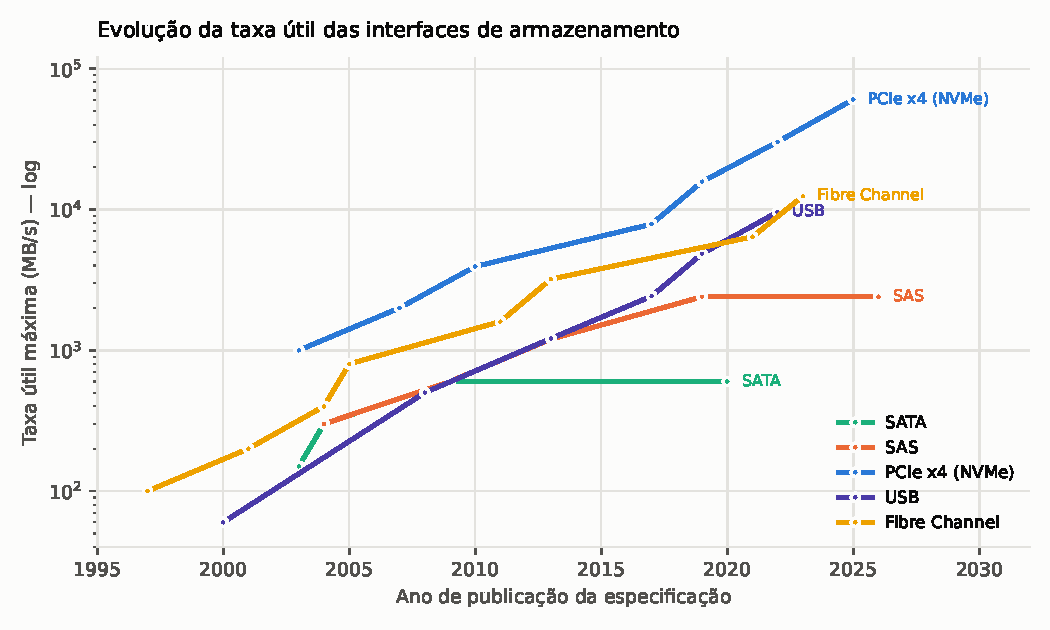
\includegraphics[width=0.80\textwidth]{fig/fig3_interfaces.pdf}
\caption{Evolução da taxa útil máxima das principais famílias de interface (escala
logarítmica; ano de publicação da especificação, que difere em até três anos do ano de mercado
usado para FC na Tabela~\ref{tab:if}). A linha horizontal do SATA desde 2009 é a estagnação da
Seção~4.3; o PCIe manteve inclinação constante por duas décadas, e por isso as demais
interfaces acabaram construídas sobre ele.}
\end{figure}

% =====================================================================
\section{Implicações para o Gerente de Armazenamento do SBD}

O \emph{gerente de armazenamento} é o módulo do SGBD que media entre as estruturas lógicas
(relações, tuplas, índices) e o meio físico: aloca arquivos e \emph{extents}, mapeia páginas
em blocos, gerencia o \emph{buffer pool}, emite e escalona I/O e garante a durabilidade
exigida pelo gerente de transações. Cada uma dessas decisões depende dos números das
Seções~3 e~4.

\subsection{Tamanho de bloco e de \emph{extent}}

\begin{center}\small
\begin{tabular}{@{}p{2.8cm}p{2.4cm}p{9.6cm}@{}}
\toprule
\textbf{Meio} & \textbf{Bloco} & \textbf{Justificativa} \\
\midrule
HDD & 8--64\,KB & O custo é dominado pelo posicionamento ($\approx$10\,ms, Tabela~\ref{tab:161}); depois dele, ler 64\,KB a 275\,MB/s custa só $\approx$0,23\,ms. Blocos maiores amortizam a busca. \\
SSD NVMe & 4--16\,KB & Alinhar à página NAND de 4\,KB evita leitura-modificação-escrita; sem busca a amortizar, blocos maiores só desperdiçam banda no acesso aleatório. \\
Fita & $\ge$1\,MB & Meio sequencial com posicionamento de 25--121\,s; só faz sentido em unidades grandes. \\
\bottomrule
\end{tabular}
\end{center}

Em SSD, o \emph{extent} continua útil por outra razão: reduz metadados, melhora a localidade
da FTL e permite ao \emph{garbage collection} liberar blocos de apagamento inteiros.

\subsection{\emph{Buffer pool} e profundidade de fila}

O gerente de \emph{buffer} clássico supõe um dispositivo que atende uma requisição por vez. Um
SSD atende 32 ou mais em paralelo (SATA: $\approx$13\,mil IOPS a QD$=$1 contra $\approx$98\,mil
a QD$=$32). Emitir uma falta de página por vez e bloquear usa algo como $1/32$ da capacidade
do dispositivo. Extrair desempenho exige \textbf{I/O assíncrono com várias requisições em
voo} (\emph{prefetch} em varreduras, leitura antecipada de nós de índice, I/O por
\emph{worker}), o que explica a adoção de \texttt{io\_uring} e do I/O assíncrono nas versões
recentes do PostgreSQL, cujo parâmetro \texttt{effective\_io\_concurrency} informa ao
planejador quantas requisições paralelas o dispositivo suporta.

\subsection{Latência de \emph{commit}}

Um \texttt{COMMIT} exige \texttt{fsync} de um registro de \emph{log} pequeno (8--16\,KB). O
quadro mostra o limite ilustrativo $1/\text{latência}$ por \emph{thread}, sem \emph{group
commit}, \emph{cache} protegido nem paralelismo; \textbf{não} é previsão de \emph{throughput}.

\begin{center}\small
\begin{tabular}{@{}lp{4.2cm}p{4.2cm}@{}}
\toprule
\textbf{Meio do \emph{log}} & \textbf{Escrita síncrona} & \textbf{Teto de \emph{commits}/s por \emph{thread}} \\
\midrule
HDD 7.200\,rpm (sem NVRAM)   & $\approx$8\,ms       & $\approx$125 \\
SSD SATA                     & $\approx$150\us & $\approx$6.700 \\
SSD NVMe local               & $\approx$30\us  & $\approx$33.000 \\
NVMe/TCP (remoto)            & $\approx$122\us{} (P99,99 WD) & $\approx$8.200 \\
iSCSI 10\,GbE                & $\approx$600\us{} (estimativa) & $\approx$1.700 \\
SCM / Optane (hipotético)    & $\approx$10\us  & $\approx$100.000 \\
\bottomrule
\end{tabular}
\end{center}
{\footnotesize Valores de ordem de grandeza. O \texttt{fsync} inclui \emph{flush}, por isso é
maior que o inverso dos IOPS de escrita da Tabela~\ref{tab:161} (28\us{} no SSD SATA, com
\emph{cache} SLC).\par}

Nenhum aumento de banda do SATA resolveria esse teto, que é de latência, e foi isso que o
NVMe atacou. A linha do SCM mostra o que a descontinuação do Optane tirou da mesa, o que faz
dessa ausência o achado mais consequente para bancos transacionais. O \textbf{\emph{group
commit}}, que agrupa vários \texttt{COMMIT}s num único \texttt{fsync}, segue sendo a mitigação
essencial.

\subsection{O modelo de custo do otimizador envelheceu}

Garcia-Molina, Ullman \& Widom (Cap.~13) formalizam o \textbf{\emph{I/O model of
computation}}: o custo de uma operação sobre disco é dominado pelo número de acessos a bloco,
e a CPU pode ser desprezada. A premissa tinha base quantitativa: um acesso a disco
($\approx$10\,ms) custava sete ordens de grandeza mais que uma instrução ($\approx$1\,ns). Com
NVMe a $\approx$50\us, a distância cai para menos de cinco ordens, e o custo de CPU do próprio
caminho de I/O (chamada de sistema e \emph{driver}, $\approx$3--7\us{} dos 23--78\us{} da
Seção~4.4) deixa de ser desprezível. O modelo não ficou falso; ficou \textbf{menos dominante}.

Em HDD, a razão entre acesso sequencial e aleatório é da ordem de 1:100, o que sustenta a regra
de que a varredura completa vence o índice quando a seletividade passa de $\approx$5--10\%. Em
NVMe essa razão cai para 1:1 a 1:3, e \textbf{o ponto de equilíbrio desloca-se a favor do
índice}.

\destaque{Onde isso aparece na prática}{%
O PostgreSQL expõe o modelo em \texttt{seq\_page\_cost} (padrão 1,0) e \texttt{random\_page\_cost}
(padrão \textbf{4,0}, premissa de disco magnético). Para SSD, a recomendação corrente é
\textbf{1,1--1,5}; sem esse ajuste, o planejador prefere varreduras que o hardware já não
favorece.}

\subsection{\emph{Tiering} automatizado de armazenamento}

Elmasri \& Navathe (§16.11.4) descrevem o \emph{automated storage tiering}: mover dados entre
meios conforme a frequência de acesso. Com os números de 2026:

\begin{center}\small
\begin{tabular}{@{}p{2.4cm}p{3.5cm}p{3.1cm}p{5.7cm}@{}}
\toprule
\textbf{\emph{Tier}} & \textbf{Meio} & \textbf{Interface} & \textbf{Conteúdo típico} \\
\midrule
0 --- memória & DRAM $+$ CXL & DDR5 / CXL 2.0 & \emph{Buffer pool}, \emph{hash}, catálogo \\
1 --- quente & SSD NVMe TLC (E3.S) & PCIe 5.0 $\times$4 & \emph{Redo log}, \texttt{tempdb}, índices, OLTP \\
2 --- morno & SSD NVMe QLC & PCIe 4.0 $\times$4 & Partições históricas, leitura intensiva \\
3 --- frio & HDD \emph{nearline} 30\,TB & SATA ou NL-SAS 12G & \emph{Data lake}, partições antigas, \emph{backup} \\
4 --- arquivo & Fita LTO-10 & SAS 12G / FC 32G & Retenção legal, \emph{air gap} \\
\bottomrule
\end{tabular}
\end{center}

Pela Tabela~\ref{tab:161}, o preço por byte do \emph{tier}~1 é $\approx$120$\times$ o do
\emph{tier}~4 ($1{,}1\times10^{-6}$ contra $9{,}3\times10^{-9}$), e o do \emph{tier}~0 (DRAM de
servidor) é $\approx$4.400$\times$. É essa razão, mais que a diferença de desempenho, que
sustenta economicamente o \emph{tiering}.

\subsection{Evidência empírica e direções emergentes}

Duas medições públicas em PostgreSQL ilustram o efeito: no Azure AKS, uma VM de 8~vCPU com NVMe
local atinge $\approx$400 mil IOPS, que com disco de rede (\emph{Ultra Disk}) exigiriam 112~vCPU
(14$\times$); e num TPC-C da Ubicloud, NVMe local, Aurora e RDS/EBS~gp3 fizeram 873, 636 e
188 transações/s, com latências de 314, 601 e 2.406\,ms (4,6$\times$ mais vazão e 7,7$\times$
menos latência que o RDS; medição de fornecedor sobre a própria plataforma). Num regime de
muitos I/Os pequenos e sincronizados, o que determina a vazão é
\textbf{latência\,$\times$\,paralelismo}, não MB/s.

Entre as direções emergentes estão o \textbf{ZNS} (NVMe~2.0), que expõe zonas do \emph{flash}
e elimina o \emph{garbage collection} do dispositivo, casando com LSM-trees; o \textbf{KV-SSD},
com interface chave-valor no lugar de blocos; o \textbf{\emph{computational storage}}, que
filtra dados dentro do SSD; o \textbf{CXL como \emph{tier} de \emph{buffer pool}}, guiado pela
\emph{Hot-Page Monitoring Unit}; o \textbf{GPUDirect Storage}; e o \textbf{NVMe~2.4}
(jul./2026), com criptografia pós-quântica e migração nativa de SSD local.

% =====================================================================
\section{Conclusão}

A hierarquia de armazenamento dos livros-texto continua existindo e governada pelo mesmo
princípio econômico, mas \textbf{os valores dos parâmetros mudaram o bastante para invalidar
várias conclusões práticas} derivadas deles.

\textbf{Primeiro}, a memória persistente endereçável por byte, apresentada como tendência nos
dois livros, \textbf{deixou de existir comercialmente}. O CXL cobre o vão entre DRAM e SSD só
em parte e só do lado volátil, a 214--271\,ns medidos, e o teto de \emph{commits} por
\emph{thread} continua fixado pela latência do NVMe.

\textbf{Segundo}, SSD e HDD \textbf{divergiram em custo por terabyte} (7$\times$ no 3T25,
23,2$\times$ no 1T26, 18,6$\times$ em 05/09/2026). O \emph{tiering}, que o SSD barato
tornaria desnecessário, ficou mais importante.

\textbf{Terceiro}, e mais relevante para a disciplina, \textbf{latência, vazão e
profundidade de fila precisam ser analisadas juntas}. Como $\approx$90\% da latência de uma
leitura em NVMe local é mídia e menos de 1\us{} é barramento, explicam-se de uma vez a
estagnação indolor do SATA em 6\,Gb/s, a vitória do NVMe sem ser mais rápido por \emph{lane}
que o SAS e a irrelevância do PCIe~6.0 para a latência de um SGBD transacional.

\textbf{Quarto}, a fita, tratada como residual, mostrou a maior vitalidade de \emph{roadmap}
da hierarquia (LTO-10 a 40\,TB nativos, US\$\,5--10/TB de mídia), ainda que o próprio
\emph{roadmap} tenha sido revisado para baixo em novembro de 2025.

Por fim, atualizar a Tabela~16.1 revelou que \textbf{os fabricantes publicam cada vez menos
parâmetros de latência}: a Seagate retirou o tempo de busca do manual do Exos~M, fabricantes de
SSD de consumo não publicam latência e a Samsung não publica IOPS do PM1743. Um trabalho
equivalente em 2014 teria mais dados disponíveis do que em 2026.

% =====================================================================
\section{Dúvidas, considerações e pontos para o debate}

\begin{enumerate}[label=\textbf{Q\arabic*.}]
\item Se \texttt{random\_page\_cost} precisa ir de 4,0 a 1,1 conforme o meio, o SGBD não
      deveria medir essa razão na inicialização? E faz sentido continuar ensinando um modelo de
      custo baseado só em contagem de blocos, sem profundidade de fila?
\item A descontinuação do Optane foi falha de mercado ou de tecnologia? Se foi custo de
      fabricação, o que impede que o vão entre DRAM e SSD fique aberto indefinidamente?
\item Se a memória barata escalar via CXL, bancos em memória de dezenas de terabytes ficam
      viáveis. O que mudaria num SGBD que hoje supõe que os dados não cabem na memória?
\item A otimização de consultas usa custo esperado (média), mas SLAs são escritos em P99 e
      P99,9. Existe formalismo que otimize percentil?
\item Armazenamento em nuvem é aceitável para o \emph{tier}~1? A degradação de 4,6$\times$ no
      TPC-C citado vem de limite físico ou de arquitetura?
\item O enunciado afirma que ``SATA também é conhecida como NL-SAS''. O grupo documentou a
      correção em vez de reproduzir a afirmação. Essa é a conduta esperada num trabalho
      avaliativo?
\end{enumerate}

% =====================================================================
\section{Referências}
\begingroup\small

\subsection*{Livros-texto}
\begin{enumerate}[label={[\arabic*]},leftmargin=*]
\item ELMASRI, R.; NAVATHE, S. B. \emph{Sistemas de Banco de Dados}. 7.\ ed. São Paulo:
      Pearson, 2018. Cap.~16 (Seções 16.1--16.3, 16.10 e 16.11; Tabela 16.1).
\item SILBERSCHATZ, A.; KORTH, H. F.; SUDARSHAN, S. \emph{Sistemas de Banco de Dados}.
      7.\ ed. Rio de Janeiro: Gen/LTC, 2020. Cap.~12 (Seções 12.1--12.7; Figura 12.1; Nota 12.1).
\item GARCIA-MOLINA, H.; ULLMAN, J. D.; WIDOM, J. \emph{Database Systems: The Complete
      Book}. 2.\ ed. Pearson, 2008. Cap.~13 --- \emph{Secondary Storage Management}.
\end{enumerate}

\subsection*{Especificações e organismos normatizadores}
\begin{enumerate}[label={[\arabic*]},leftmargin=*,start=4]
\item PCI-SIG. \emph{PCI Express Base Specification 7.0}, 11/jun./2025. \url{https://pcisig.com}
\item NVM EXPRESS. \emph{NVM Express Base Specification} 1.0 (2011) a 2.4 (2026).
      \url{https://nvmexpress.org/specification/nvm-express-base-specification/}
\item NVM EXPRESS. \emph{NVMe over Fabrics} 1.0 (2016) e 1.1 (2019).
\item SATA-IO. \emph{Serial ATA Specification Revision 3.5} (2020). \url{https://sata-io.org}
\item INCITS/T10. \emph{SAS-4} e projeto SAS-5 (BSR INCITS 561). \url{https://www.t10.org}
\item INCITS/T11 e FCIA. \emph{Fibre Channel Roadmap}; FC-PI-8 (INCITS 560-2023).
      \url{https://fibrechannel.org}
\item IBTA. \emph{InfiniBand Architecture Specification}; anúncio XDR, out./2023.
      \url{https://infinibandta.org}
\item IETF. \emph{RFC 7143 --- iSCSI Protocol (Consolidated)}, abr./2014.
      \url{https://www.rfc-editor.org/rfc/rfc7143.html}
\item USB-IF. \emph{USB4 Version 2.0 Specification}. \url{https://www.usb.org/usb4}
\item CXL CONSORTIUM. \emph{Compute Express Link} 3.1 (nov./2023) e 3.2 (dez./2024).
\item SNIA. \emph{EDSFF Form Factors} (SFF-TA-1006/1007/1008); \emph{What is NVMe-oF}.
      \url{https://www.snia.org}
\item ULTRA ETHERNET CONSORTIUM. \emph{UEC Specification 1.0}, jun./2025.
\item LTO PROGRAM. \emph{LTO-9 Technical Brief}; \emph{LTO Program Announces New 40\,TB LTO-10
      Cartridge Specifications and Refreshes its Roadmap}, 12/nov./2025 (913\,TB comprimidos
      no LTO-14 $=$ 365\,TB nativos a 2,5:1; Seção~2.6).
      \url{https://www.lto.org/2025/11/lto-program-announces-new-40-tb-lto-10-cartridge-specifications-and-refreshes-its-roadmap-for-ultra-high-density-ai-ready-archival-storage/}
\end{enumerate}

\subsection*{Documentação de fabricante}
\begin{enumerate}[label={[\arabic*]},leftmargin=*,start=17]
\item AMD. \emph{Ryzen 9 9950X3D2 Dual Edition --- Specifications}.
      \url{https://www.amd.com/en/products/processors/desktops/ryzen/9000-series/amd-ryzen-9-9950x3d2-dual-edition.html}
\item SEAGATE. \emph{Exos M SATA Product Manual, 32/30/28/24\,TB}, Rev.~D, ago./2025; e
      \emph{Seagate Introduces Hard Drive Capacities of Up to 36TB}, 20/jan./2025 (ponto de 36\,TB).
      \url{https://investors.seagate.com/news/news-details/2025/Seagate-Introduces-Hard-Drive-Capacities-of-Up-to-36TB-Extending-Its-HAMR-Based-Mozaic-3-Technology-Platform/default.aspx}
\item SOLIDIGM. \emph{D5-P5336 Product Specification}.
\item MICRON. \emph{9550 PRO NVMe SSD}; \emph{9650 Series} (PCIe~6.0, produção desde fev./2026).
\item SAMSUNG. \emph{SSD 870 EVO Data Sheet} Rev.~1.1
      (\url{https://download.semiconductor.samsung.com/resources/data-sheet/Samsung_SSD_870_EVO_Data_Sheet_Rev1.1_230509_10129500053000.pdf});
      \emph{9100 PRO Data Sheet} Rev.~1.0
      (\url{https://download.semiconductor.samsung.com/resources/data-sheet/Samsung_NVMe_SSD_9100_PRO_Datasheet_Rev.1.0_10149294091048.pdf})
      e anúncio de MSRP
      (\url{https://news.samsung.com/us/samsung-announces-9100-pro-series-ssds-with-breakthrough-pcie-5-0-performance/});
      \emph{CMM-D MD220}.
\item KIOXIA. \emph{CM9-R Product Brief}.
\item WESTERN DIGITAL. \emph{NVMe-oF Network Storage Protocol: NVMe/TCP vs.\ RDMA with RoCEv2}
      (OpenFlex Data24); 4\,K aleatório, QD1, 1 \emph{job}, 20\,min, ``measured at the 4 nines''.
      \url{https://documents.westerndigital.com/content/dam/doc-library/en_us/assets/public/western-digital/collateral/white-paper/white-paper-open-flex-data24-roce-vs-tcp.pdf}
\item BROADCOM. \emph{Brocade G720 Switch Product Brief} (460\,ns para portas comutadas
      localmente, incluindo FEC). \url{https://docs.broadcom.com/doc/G720-Switch-PB};
      \emph{eHBA 9600-24i}; \emph{Emulex LPe38102}.
\item MARVELL. \emph{QLogic 2870 Series 64GFC Fibre Channel HBA}.
\item NVIDIA. \emph{Magnum IO GPUDirect Storage}; \emph{Quantum InfiniBand Switches}.
\item IBM. \emph{TS4500 Tape Library}.
      \url{https://www.ibm.com/docs/en/ts4500-tape-library/1.12.2?topic=overview-introduction-ts4500-tape-library};
      QUANTUM. \emph{Scalar i6000}.
\item VERBATIM. \emph{M-DISC BDXL 100\,GB}; PIONEER. \emph{BDR-X13U-S}.
\end{enumerate}

\subsection*{Mercado e medições de terceiros}
\begin{enumerate}[label={[\arabic*]},leftmargin=*,start=29]
\item TRENDFORCE. Relatórios de preço de contrato de DRAM e NAND, 1T26 a 3T26 (série de
      contexto; sem valores pontuais no texto). \url{https://www.trendforce.com/price}
\item VDURA. \emph{Flash Volatility Index} --- ``SSD Prices Settle Into a Costly New Normal at
      $\sim$6.5x Year-Ago Levels'', 11/ago./2026 (18,6$\times$, 23,2$\times$, 7,0$\times$;
      US\$\,22.600 e US\$\,1.216).
      \url{https://www.vdura.com/2026/08/11/ssd-prices-settle-into-a-costly-new-normal-at-6-5x-year-ago-levels-reshaping-the-economics-of-ai-factories-vdura-flash-volatility-index-shows/}
\item MICROSOFT AZURE. \emph{PostgreSQL on AKS with local NVMe}, jul./2025.
      \url{https://techcommunity.microsoft.com/category/azure/blog/adforpostgresql}
\item UBICLOUD. \emph{PostgreSQL performance: local vs.\ network-attached storage} (medição do
      próprio fornecedor). \url{https://www.ubicloud.com/blog}
\item SCSI TRADE ASSOCIATION / SNIA. \emph{SAS Technology Roadmap}; declarações sobre 24G$+$ e
      SAS-5. \url{https://www.snia.org/forums/sfa}
\item Medição revisada por pares de latência de expansores CXL~2.0 (214--271\,ns contra
      111--117\,ns de DDR5 local). Referência exata ainda não fixada pelo grupo; valores
      tratados como ordem de grandeza (Nota~N5).
\end{enumerate}
\endgroup

\clearpage
% =====================================================================
\section{Post-Mortem --- Uso de Assistentes de IA Generativa}

Esta seção atende ao enunciado com (i)~o log dos prompts-chave, (ii)~a demonstração de
autoria e (iii)~o registro dos erros gerados pela IA e das correções. Ela documenta o que foi
verificado e como, separando dado de fonte, estimativa e lacuna.

\subsection{Ferramentas utilizadas}

\begin{center}\small
\begin{tabular}{@{}p{4.2cm}p{5.4cm}p{4.4cm}@{}}
\toprule
\textbf{Ferramenta} & \textbf{Uso} & \textbf{Limitação observada} \\
\midrule
Assistente de IA generativa com busca web & Levantamento de \emph{datasheets}, normas e preços; primeira redação das seções expositivas & Fontes de preço divergentes; estimativas apresentadas com a confiança de dados publicados \\
Segunda instância de IA, modo adversarial & Verificação de 29 afirmações contra fonte primária (Seção~9.5) & Sem instrução explícita, tende a confirmar o que soa plausível \\
Codex & Conferência de consistência (06/09) e revisão editorial (08/09) & Verificou aritmética e coerência; não reconfirmou fontes comerciais \\
Claude & Revisão de condensação e coerência interna (11/09) & Idem; achados E22--E26 \\
\texttt{pdftotext}, Python/Matplotlib, \LaTeX & Leitura dos capítulos, cálculo do preço por KB, figuras e diagramação & Cálculos conferidos por amostragem \\
\bottomrule
\end{tabular}
\end{center}

\subsection{Log dos \emph{prompts}-chave}

Prompts de ajuste estilístico foram omitidos.

\begin{enumerate}[label=\textbf{P\arabic*.},leftmargin=*]
\item \textbf{Extração da base textual.} ``Leia os capítulos anexos (Elmasri cap.~16 e
      Silberschatz cap.~12). Extraia a Tabela~16.1 original na íntegra, com todas as colunas e
      valores, e os parâmetros de desempenho de disco e de flash discutidos no texto.''\\
      \emph{Papel:} partir do original exato, não de reconstrução de memória do modelo.
\item \textbf{Levantamento de dispositivos.} ``Para cada categoria da Tabela~16.1 (cache, DRAM,
      SCM, SSD NVMe consumidor e datacenter, SSD SATA, pen drive, HDD, óptico, fita, tape
      library), encontre 1--2 produtos comerciais específicos com marca e modelo e reporte
      capacidade, tempo de acesso, largura de banda de leitura e de escrita separadas, e preço
      atual, com URL da fonte. Marque claramente o que vem de datasheet oficial, o que é
      medição de terceiro e o que é estimativa. Não invente; se não encontrar, diga que não
      encontrou.''\\
      \emph{Papel:} a exigência de marcar a origem de cada número foi a decisão metodológica
      mais importante do trabalho.
\item \textbf{Levantamento de interfaces.} ``Para USB (1 a 4), SCSI, SATA (1--3), eSATA, SATA
      Express, NVMe/PCIe, M.2, U.2, SAS (1--4), iSCSI, FireWire, HBA, FC (incluindo FCIP e
      FCoE) e InfiniBand, reporte ano da especificação, serial ou paralela, taxa bruta e taxa
      útil, latência típica, distância máxima, portabilidade, topologia e número máximo de
      dispositivos, com fontes normativas. Distinga rigorosamente Gb/s de GB/s e cite a
      codificação de linha que explica a diferença.''\\
      \emph{Papel:} forçou a distinção entre taxa bruta e útil em toda a Tabela~\ref{tab:if}.
\item \textbf{Verificação de afirmação do enunciado.} ``O enunciado afirma que `SATA também é
      conhecida como NL-SAS'. Verifique se isso é correto e reporte a correção com fontes.''\\
      \emph{Papel:} testar uma suspeita levantada pelo grupo na leitura de Elmasri (Seção~4.3).
\item \textbf{Anomalia de preços.} ``Há relatos de alta de preço de memória em 2025--2026 por
      demanda de IA. Verifique se procede e quantifique com fontes de mercado.''\\
      \emph{Papel:} evitar apresentar preços de pico como tendência estrutural.
\item \textbf{Lacunas.} ``Liste explicitamente o que você NÃO conseguiu encontrar em fonte
      pública.''\\
      \emph{Papel:} produziu a Nota~N8; tratar lacuna como resultado foi decisão do grupo.
\item \textbf{Verificação adversarial.} ``Você é um verificador de fatos adversarial. Verifique
      cada afirmação abaixo com busca web e classifique como CONFIRMADO (com fonte), IMPRECISO
      (explique o que está errado e qual o valor correto), NÃO VERIFICÁVEL ou FALSO. Seja
      implacável: o objetivo é encontrar erros ANTES que um professor os encontre. Não confirme
      nada por plausibilidade --- só com fonte. Se não achar fonte, diga NÃO VERIFICÁVEL, o que
      já é um achado. Ao final, ordene por gravidade o que um professor rigoroso poderia usar
      para derrubar o trabalho.''\\
      \emph{Papel:} o prompt com melhor razão entre erros encontrados e esforço (E13--E21).
\item \textbf{Condensação e coerência (11/09).} ``De acordo com a descrição do trabalho, o que a
      gente poderia diminuir no relatório de modo a continuar atendendo a todos os requisitos da
      descrição, manter uma boa qualidade no relatório e completude, mas diminuindo volume pois
      está muito grande. Poderia aplicar uma grande correção nesse trabalho analisando isso.''\\
      \emph{Papel:} reduziu repetições (o mesmo fato aparecia em até cinco lugares), agrupou
      versões na Tabela~\ref{tab:if} e expôs as inconsistências E22--E26.
\end{enumerate}

\subsection{Demonstração de autoria --- quem fez o quê e por quê}

\begin{center}\small
\begin{tabular}{@{}p{3.3cm}p{4.3cm}p{7.2cm}@{}}
\toprule
\textbf{Integrante} & \textbf{Responsabilidade} & \textbf{Decisões e justificativa} \\
\midrule
Bernardo Brandão Pozzato Carvalho Costa & Coordenação; Seções 1 e 6; revisão final & Adotou faixas de preço em vez de pontos, pela divergência entre rastreadores; incluiu o aviso sobre a crise de preços de 2026. \\
Enzo de Carvalho Sampaio & Seção 2; leitura dos capítulos-base & Articulou os dois livros-texto: Elmasri para arquiteturas modernas, Silberschatz para \emph{flash} e FTL. \\
Gabriel Schmitz Corrêa Rizawinsk & Seção 3; cálculo do preço por KB & Documentou as convenções de unidade; acrescentou e justificou as linhas novas (CXL, SSD \emph{datacenter}, LTO-10). \\
Vivian Maria da Silva e Souza & Seção 4; verificação normativa & Adotou taxa por direção no FC para comparabilidade; detectou e documentou a correção sobre NL-SAS. \\
Raphael Henrique da Silva Pereira & Seção 5; coordenação da consolidação do Post-Mortem (06/09) e da revisão editorial (08/09), executadas com o Codex & Ancorou a discussão em parâmetros reais de SGBD (\texttt{random\_page\_cost}, \texttt{effective\_io\_concurrency}); separou problemas corrigidos de pendências. \\
Guilherme En Shih Hu & Rodada adversarial; revisão final dos artefatos & Manteve uma segunda rodada independente e só fechou a entrega com contas e termos coincidindo entre relatório e slides. \\
\bottomrule
\end{tabular}
\end{center}

\textbf{Nota de honestidade acadêmica.} A redação inicial de várias seções expositivas foi
produzida por IA a partir dos prompts acima. Os integrantes definiram escopo e estrutura,
verificaram números contra fonte primária, corrigiram os erros da Seção~9.4 e escreveram as
análises interpretativas. As revisões assistidas de 06/09, 08/09 e 11/09 conferiram
aritmética e coerência, mas não constituem nova confirmação humana das fontes comerciais.

\subsection{Erros gerados pela IA e correções aplicadas}

{\small
\setlength{\tabcolsep}{4pt}
\begin{longtable}{@{}p{0.7cm}>{\RaggedRight\arraybackslash}p{5.5cm}>{\RaggedRight\arraybackslash}p{5.6cm}>{\RaggedRight\arraybackslash}p{2.8cm}@{}}
\caption{Registro de erros e correções.}\label{tab:erros}\\
\toprule
\textbf{\#} & \textbf{Erro gerado} & \textbf{Correção aplicada} & \textbf{Detecção} \\
\midrule
\endfirsthead
\toprule
\textbf{\#} & \textbf{Erro gerado} & \textbf{Correção aplicada} & \textbf{Detecção} \\
\midrule
\endhead
\bottomrule
\endfoot
E1 & Preço da SRAM (delta de V-Cache) apresentado como preço de mercado. & Reclassificado como \emph{proxy} (Nota N2). & Gabriel, ao reproduzir a conta. \\
E2 & Mistura de convenção binária e decimal na SRAM ($\approx$5\% de divergência). & Convenção fixada por categoria e valores recalculados em script único (Seção~1.2). & Gabriel, ao verificar 199/64\,MiB. \\
E3 & Sugeriu manter o Intel Optane na tabela. & Linha removida pelo critério C2; ausência tratada como achado (Seção~2.5). & Bernardo. \\
E4 & LTO-10 com 36, 30 e 40\,TB em trechos diferentes. & Cronologia reconstruída: 36\,TB era meta antiga; 30\,TB no lançamento; 40\,TB no cartucho de 2026. & Gabriel. \\
E5 & 64GFC como ``12.800\,MB/s'' sem qualificar. & Valor da FCIA é \emph{full-duplex}; adotados 6.400\,MB/s por direção. & Vivian. \\
E6 & SAS-4 como ``24\,Gb/s''. & 22,5\,Gb/s (``24G'' é marca); taxa útil 2.400\,MB/s com 128b/150b. & Vivian. \\
E7 & Ecoou ``SATA também é conhecida como NL-SAS''. & Verificação dirigida (P4); correção destacada na Seção~4.3. & Vivian, na leitura de Elmasri. \\
E8 & Tempo de busca do Exos~M como dado de \emph{datasheet}. & A Seagate removeu o \emph{seek time} do manual. Primeiro remarcado como estimativa; na revisão de 08/09, substituído pelos 10\,ms do livro (N4). & Gabriel. \\
E9 & DRAM de servidor a US\$\,37,31/GB e US\$\,4,47/GB sem sinalizar contradição. & Rastreadores com metodologias distintas; adotada faixa (N7). & Bernardo. \\
E10 & \emph{Throughput} de biblioteca de fita como especificação. & IBM e Quantum não publicam; derivação marcada como teto teórico (N6). & Guilherme. \\
E11 & Mesmo valor nas colunas de leitura e escrita para todos os meios. & Segregação onde há dado (ex.: Solidigm 7,0 contra 3,0\,GB/s); meios simétricos indicados. & Gabriel. \\
E12 & Latências estimadas de SSD de consumo com a confiança de dados publicados. & Marcação de origem em toda a tabela; na revisão de 08/09, valores não confirmados trocados pelos 50\us{} do livro (N4). & Enzo. \\
\multicolumn{4}{@{}l}{\emph{Detectados na rodada adversarial (Seção~9.5):}}\\
E13 & ``913\,TB nativos no LTO-14''. & São 913\,TB comprimidos (365\,TB nativos), e de \emph{roadmap} já revisado em nov./2025. & Adversarial; confirmado por Gabriel. \\
E14 & Latência de $\approx$140\,ns para o CMM-D. & Sem fonte; adotados 214--271\,ns medidos (N5). & Adversarial. \\
E15 & Razão SSD/HDD ``$\approx$16$\times$ em 2026'' sem trimestre. & Tabela por período e data em todas as ocorrências (Seção~3.4). & Adversarial. \\
E16 & Alta do HDD ``46--50\% em seis meses'' e NAND ``5$\times$ entre ago./2025 e jan./2026''. & Janelas corrigidas: HDD $+$46\% em quatro meses; NAND 5$\times$ desde out./2025, 8,5$\times$ em mar./2026. Trecho posteriormente retirado do corpo. & Adversarial. \\
E17 & Resumo citava ``trinta e nove variantes'' de interface. & Contagem refeita contra a tabela; na versão condensada, versões agrupadas em 32 linhas e o resumo deixou de citar número. & Adversarial. \\
E18 & Confundiu latência típica e QoS do D5-P5336. & Valores não confirmados retirados; adotados os 50\us{} do livro (N4). & Revisão assistida por IA. \\
E19 & Latências da Western Digital rotuladas como ``medidas'' e ``total observado''. & São P99,99; rótulo corrigido na Tabela~\ref{tab:if}, na Seção~4.3 e no orçamento de latência. & Adversarial. \\
E20 & Capacidades diferentes do 9100 PRO na mesma linha. & Linha fixada no modelo de 1\,TB (N1); taxas do M-DISC corrigidas. & Adversarial. \\
E21 & Ciclos de L2/L3 do Zen~5 tratados como publicados; conversão sem \emph{clock}. & Derivação completa com \emph{clock} declarado de 5,6\,GHz (N3). & Adversarial. \\
\multicolumn{4}{@{}l}{\emph{Inconsistências detectadas na revisão de condensação (11/09/2026):}}\\
E22 & Contas internas que não fechavam: ``$\approx$134\,PB'' para 0,6~DWPD em 61,44\,TB; ``vazio de cinco ordens'' na legenda da Figura~1; razão de preço \emph{tier}~1/\emph{tier}~4 de ``20--40$\times$''. & Recalculados: $\approx$67\,PB; quase três ordens; $\approx$120$\times$ pela própria Tabela~\ref{tab:161}. & Revisão assistida por IA. \\
E23 & Orçamento de latência com parcelas que não somavam o total e totais misturando média e P99,99; NVMe/TCP ``80--150\us{} acima do RoCE'' e RoCE recomendado ``para P99 abaixo de 150\us''. & Soma das estimativas separada da medição WD; diferença medida corrigida para 14--81\us; recomendação reescrita (a leitura P99,99 do RoCE é 162,8\us). & Revisão assistida por IA. \\
E24 & Referências cruzadas quebradas: ``Seção 4.3.12'', ``Seção 3.3'', ``Nota N10'' (lista com seis itens descrita como ``dez''), ref.~[16] apontando a Seção 3.4, citação a material da Dell ausente das referências e numeração [28] duplicada. & Remissões refeitas, notas renumeradas (N1--N8), menção à Dell retirada e referências renumeradas de [1] a [34]. & Revisão assistida por IA. \\
E25 & Correções locais que criaram contradições remotas: \emph{clock} de 5,6\,GHz (N3) contra 5,7\,GHz (E21); E8 e E12 descrevendo notas já alteradas; busca de ``12,7\,ms'' e taxa de 285\,MB/s na Seção~5 contra 10\,ms e 275\,MB/s da tabela; ``quatro linhas novas'' descritas como três. & Valores alinhados à Tabela~\ref{tab:161}; descrições de E8, E12 e E21 atualizadas. & Revisão assistida por IA. \\
E26 & Origem da frase sobre NL-SAS atribuída a Elmasri §16.2.1 (Q7) e §16.11 (P4, E7). & Remissão neutralizada para ``Elmasri'' até conferência da página no livro. & Revisão assistida por IA. \\
\end{longtable}
}

\subsection{A rodada de verificação adversarial}

Com a primeira versão completa, o grupo submeteu 29 afirmações verificáveis (produtos,
cronologia, mercado e taxas) a uma segunda IA com busca web e instrução de derrubar o
trabalho: classificar cada afirmação como confirmada (com URL), imprecisa (com o valor
correto), não verificável ou falsa; \textbf{não confirmar por plausibilidade}; tratar ausência
de fonte como achado; e ordenar por gravidade. A primeira IA, autora do texto, era a menos
indicada para auditá-lo.

\begin{center}\small
\begin{tabular}{@{}lcp{10.2cm}@{}}
\toprule
\textbf{Veredito} & \textbf{Qtd.} & \textbf{Exemplos} \\
\midrule
Confirmada & 15 & Ryzen 9 9950X3D2 (192\,MB de L3); remoção do \emph{seek time} do Exos~M; datas do Optane; PCIe~7.0 em 11/06/2025; 460\,ns do G720; PAM3 no USB4 v2.0 \\
Imprecisa & 9 & Roadmap do LTO; janelas de preço; razão SSD/HDD sem data; QoS do Solidigm; ciclos de \emph{cache} do Zen~5 \\
Não verificável & 4 & Latência do CMM-D; taxa do SAS-5; leitura do M-DISC; banda do MD220 \\
Falsa & 1 & ``913\,TB nativos no LTO-14'' \\
\bottomrule
\end{tabular}
\end{center}

Nove achados geraram as correções E13--E21: cinco de conteúdo (E13--E17) e quatro de
\textbf{rótulo} (E18--E21), em que o número existia, mas descrevia outra coisa (QoS como
latência típica, percentil como média, capacidades misturadas, derivação como especificação).
Esses últimos são os mais insidiosos, porque passam numa busca simples. As quatro afirmações
não verificáveis passaram de afirmação a estimativa declarada.

\subsection{Lições aprendidas}

\begin{enumerate}[label=\textbf{L\arabic*.},leftmargin=*]
\item \textbf{Exigir a origem de cada número} (P2) tornou o trabalho auditável, e pedir as
      lacunas explicitamente (P6) evitou que o assistente as preenchesse.
\item \textbf{A IA reproduz premissas erradas do próprio pedido}: E7 só apareceu porque o grupo
      desconfiou do enunciado. A verificação contra fonte primária vale para qualquer autor,
      inclusive o livro-texto (Silberschatz grafa ``6 gigabytes per second'' para o SATA-3).
\item \textbf{Autoria e auditoria precisam ser papéis separados}: os cinco erros de conteúdo
      mais graves sobreviveram à revisão da IA autora e caíram na primeira passagem do
      verificador adversarial. Se houver uma prática a levar para o uso profissional de IA, é
      esta.
\item \textbf{Número sem data ou sem rótulo não é dado} (E15, E19): em mercados voláteis a data
      faz parte do valor, e um percentil sem rótulo muda a conclusão.
\item \textbf{Cada rodada de correção pode quebrar outra parte do texto}: E25 reúne
      contradições criadas por correções feitas em um trecho sem propagar aos demais. Depois de
      cada revisão, é preciso reler o documento cruzando seções, não só o trecho alterado.
\item \textbf{O trabalho interpretativo permaneceu humano}: as conclusões da Seção~6 vieram de
      comparar tabelas produzidas separadamente, não de respostas prontas do assistente.
\end{enumerate}

% =====================================================================
\section*{Anexo A --- Glossário de siglas}
\addcontentsline{toc}{section}{Anexo A --- Glossário de siglas}

{\small
\noindent
\begin{minipage}[t]{0.49\textwidth}
\begin{tabular}[t]{@{}l>{\RaggedRight\arraybackslash}p{4.4cm}@{}}
\toprule
\textbf{Sigla} & \textbf{Significado} \\
\midrule
AHCI & Advanced Host Controller Interface \\
CXL & Compute Express Link \\
DWPD & Drive Writes Per Day \\
EDSFF & Enterprise and Data Center Standard Form Factor \\
FC / FCIP / FCoE & Fibre Channel; sobre IP; sobre Ethernet \\
FTL & Flash Translation Layer \\
HAMR & Heat-Assisted Magnetic Recording \\
HBA & Host Bus Adapter \\
IOPS & Input/Output Operations Per Second \\
LTO & Linear Tape-Open \\
MTTF & Mean Time To Failure \\
NCQ / TCQ & Native / Tagged Command Queuing \\
NL-SAS & Nearline SAS \\
\bottomrule
\end{tabular}
\end{minipage}\hfill
\begin{minipage}[t]{0.49\textwidth}
\begin{tabular}[t]{@{}l>{\RaggedRight\arraybackslash}p{4.4cm}@{}}
\toprule
\textbf{Sigla} & \textbf{Significado} \\
\midrule
NVMe / NVMe-oF & Non-Volatile Memory Express; over Fabrics \\
PAM3 / PAM4 & Pulse Amplitude Modulation de 3 e 4 níveis \\
QD & Queue Depth (profundidade de fila) \\
RDMA / RoCE & Remote Direct Memory Access; sobre Ethernet convergente \\
SAN / NAS & Storage Area Network / Network-Attached Storage \\
SAS & Serial Attached SCSI \\
SCM & Storage Class Memory \\
STP & Serial ATA Tunneling Protocol \\
TBW & Terabytes Written \\
UEC & Ultra Ethernet Consortium \\
WORM & Write Once, Read Many \\
ZNS & Zoned Namespaces \\
\bottomrule
\end{tabular}
\end{minipage}
}

\end{document}
